\chapter{数学物理方程}

\begin{flushright}
\textit{“致知在格物。”——《大学》}
\footnote{格物是把现象里的守恒和对称写成方程.波动、扩散和势的定解问题都从这里写起.}
\end{flushright}

这一章从物理图像写出波动、扩散和势方程,再讨论定解条件、方程类型、分离变量、行波解和积分变换.进一步的材料见~\cite{strauss,tikhonov,courant,guqiao,ivrii}.

数学物理方程是该课程的重要组成部分.
研究物理量在空间中的分布和在时间上的变化情况是物理规律要探讨的主要内容.
\section{数学物理方程的推导}
\idx{弦振动方程}{xianzhen}
\idx{热传导方程}{rechuandao}
物理规律反映的是某个物理量在邻近地点和邻近时刻之间的联系,因此数
学物理方程的导出步骤如下: 首先当然要确定研究哪一个物理量 $u$. 从所研究的系统中划出一个小部分, 
根据物理规律分析邻近部分和这个小部分的相互作
用 (抓住主要的作用, 略去不那么重要的因素), 这种相互作用在一个短时间段里怎样影响物理量 $u$.
 把这种影响用算式表达出来, 经简化整理就是数学物理方程.

下面我们以三个典型的数理方程, 波动方程、输运方程和稳定场方程为例来演示推导过程.
它们大致对应数学上二阶偏微分方程的分类,即双曲型、抛物型和椭圆型.

\subsection{弦振动方程}
\textbf{弦振动方程}是在 18 世纪由达朗贝尔 (D'Alembert) 等人首先给予系统研究的.
它是一大类偏微分方程的典型代表.下面先从物理问题出发来导出弦振动方程.

给定一根两端固定的拉紧的均匀柔软的弦, 其长为 $l$, 在外力作用下在平衡位置附近作微小的横振动, 
求弦上各点的运动规律.

将实际问题归结为数学模型时,必须作一些理想化的假设, 以便抓住问题的最本质的特征.
在考察弦振动问题时的基本假设为:
\begin{enumerate}
    \item  弦是均匀的, 弦的截面直径与弦的长度相比可以忽略, 因此弦可以视为一根曲线, 
        它的(线) 密度 $\rho$ 是常数.
    \item 弦在某一平面内作微小横振动, 即弦的位置始终在一直线段附近, 
        而弦上各点均在同一平面内垂直于该直线的方向上作微小振动.
    \item  弦是柔软的, 它在形变时不抵抗弯曲, 弦上各质点间的张力方向与弦的切线方向一致,
        而弦的伸长形变与张力的关系服从胡克(Hooke)定律.
\end{enumerate}

我们将在上述假定下来导出弦振动方程.先讨论不受外力作用时弦振动的情形.根据牛顿第二定律知
$$
\text{作用在物体上的力} = \text{该物体的质量} \times \text{该物体的加速度}
$$

于是在每一个时间段内
$$
\text{作用在物体上的冲量} = \text{ 该物体的动量的变化}.
$$

由于弦上各点的运动规律不同, 必须对弦的各个片段分别进行考察.
为此, 我们选择坐标系, 将弦的两端固定在 $x$ 轴的 $A,B$ 两点上 $(AB=l)$ .
由基本假设, 可以用 $u(x, t)$ 表示
弦上各点在时刻 $t$ 沿垂直于 $x$ 方向的位移.当 $t$ 固定时 $u(x, t)$ 即表示弦在该时刻所处的位置.


在这弦上任取一弦段 $(x, x+\Delta x)$, 它的弧长为
$$
\Delta s=\int_x^{x+\Delta x} \sqrt{1+\left(\frac{\partial u}{\partial x}\right)^2} d x,
$$

由基本假设2知 $\frac{\partial u}{\partial x}$ 很小,于是 $\left(\frac{\partial u}{\partial x}\right)^2$ 与 1 相比可以忽略不计, 从而
$$
\Delta s \approx \int_x^{x+\Delta x} d x=\Delta x
$$

这样, 可以认为这段弦在振动过程中并未伸长, 因此由胡克定律知道, 弦上每一点所受张力在运动过程中保持不变, 
即张力与时间无关.我们把在 $x$ 点处的张力记为 $\boldsymbol{T}(x)$, 它表示在 $x$ 
点处弦的左边部分对右边部分的拉力与弦的右边部分对左边部分的拉力大小均为 $T(x)$. 
由基本假设 3 知,张力 $\boldsymbol{T}(x)$ 的方向总是沿着弦在 $x$ 点处的切线方向.
 在 $x$ 点处作用于弦段 $(x, x+\Delta x)$ 的张力在 $x$, $u$ 两个方向上的分力分别为
$$
-T(x) \cos \alpha_1, \quad-T(x) \sin \alpha_1,
$$
这里 $\alpha_1$ 是张力 $\boldsymbol{T}(x)$ 的方向与水平线的夹角, 
负号表示力的方向取与坐标轴相反的方向. 在弦段的另一端 $x+\Delta x$ 点处作用于弦段 $(x, x+\Delta x)$ 
的张力在 $x$, $u$两个方向的分力分别为
$$
T(x+\Delta x) \cos \alpha_2, \quad T(x+\Delta x) \sin \alpha_2,
$$

其中 $\alpha_2$ 是张力 $\boldsymbol{T}(x+\Delta x)$ 与水平线的夹角.
由于弦只在 $x$ 轴的垂直方向作横振动, 所以水平方向的合力为零, 即
$$
T(x+\Delta x) \cos \alpha_2-T(x) \cos \alpha_1=0 .
$$

由于假设弦仅在平衡位置附近作微小振动, 所以
$$
\begin{aligned}
& \cos \alpha_1=\frac{1}{\sqrt{1+\left[\frac{\partial u(x, t)}{\partial x}\right]^2}} \approx 1, \\
& \cos \alpha_2=\frac{1}{\sqrt{1+\left[\frac{\partial u(x+\Delta x, t)}{\partial x}\right]^2}} \approx 1,
\end{aligned}
$$

$$
T(x+\Delta x)-T(x)=0,
$$

故 $T(x+\Delta x)=T(x)=T$, 也就是说, $T$ 是一个常数.又由基本假设 2 知
$$
\begin{aligned}
& \sin \alpha_1 \approx \tan \alpha_1=\frac{\partial u(x, t)}{\partial x}, \\
& \sin \alpha_2 \approx \tan \alpha_2=\frac{\partial u(x+\Delta x, t)}{\partial x},
\end{aligned}
$$

所以张力在 $x$ 轴的垂直方向的合力为
$$
T \sin \alpha_2-T \sin \alpha_1=T\left[\frac{\partial u(x+\Delta x, t)}{\partial x}-\frac{\partial u(x, t)}{\partial x}\right],
$$

从而在时间段 $(t, t+\Delta t)$ 中该合力产生的冲量为
$$
\int_t^{t+\Delta t} T\left[\frac{\partial u(x+\Delta x, t)}{\partial x}-\frac{\partial u(x, t)}{\partial x}\right] d t .
$$

另一方面, 在时刻 $t$ 弦段 $(x, x+\Delta x)$ 的动量为
$$
\int_x^{x+\Delta} \rho \frac{\partial u(x, t)}{\partial t} d x,
$$

在时刻 $t+\Delta t$ 该弦段的动量为
$$
\int_x^{x+\Delta} \rho \frac{\partial u(x, t+\Delta t)}{\partial t} d x,
$$

所以从时刻 $t$ 到时刻 $t+\Delta t$, 弦段 $(x, x+\Delta x)$ 的动量增加量为
$$
\int_x^{x+\Delta x} \rho\left[\frac{\partial u(x, t+\Delta t)}{\partial t}-\frac{\partial u(x, t)}{\partial t}\right] d x .
$$

由于在 $(t, t+\Delta t)$ 时间段内的冲量应等于动量的增加, 故
$$
\int_t^{t+\Delta t} T\left[\frac{\partial 
u(x+\Delta x, t)}{\partial x}-\frac{\partial u(x, t)}{\partial x}\right] d t
=\int_{x}^{\Delta+x} \rho\left[\frac{\partial u(x, t+\Delta t)}{\partial t}-
\frac{\partial u(x, t)}{\partial t}\right] d x,
$$

从而
\begin{equation}
\int_t^{t+\Delta t} \int_{x}^{x+ \Delta x} 
\left[T \frac{\partial^2 u(x, t)}{\partial x^2}-\rho 
\frac{\partial^2 u(x, t)}{\partial t^2}\right] d x d t=0 .
\label{eq:string_vibration}
\end{equation}

由 $\Delta x, \Delta t$ 的任意性可知 式\eqref{eq:string_vibration} 中的被积函数必须为零, 从而得到
\begin{equation}
T \frac{\partial^2 u(x, t)}{\partial x^2}-\rho \frac{\partial^2 u(x, t)}{\partial t^2}=0 .
\end{equation}


记 $\frac{T}{\rho}$ 为 $a^2$, 就得到不受外力作用时弦振动所满足的方程
\begin{equation}
\frac{\partial^2 u}{\partial t^2}-a^2 \frac{\partial^2 u}{\partial x^2}=0 .
\label{eq:free_vibration}
\end{equation}
该方程称为弦的\textbf{自由振动方程}.

当存在外力作用时, 若在点 $x$ 处外力 (线) 密度为 $F(x, t)$, 其方向垂直于 $x$ 轴, 则小弦段 $(x, x+\Delta x)$ 上所受外力为
$$
\int_x^{x+\Delta x} F(x, t) d x,
$$

它在时间段 $(t, t+\Delta t)$ 中所产生的冲量为
$$
\int_t^{t+\Delta t} \int_x^{x+\Delta } F(x, t) d x d t .
$$

于是在方程 \eqref{eq:string_vibration} 的左侧应添上这一项, 得到

$$
\int_t^{t+\Delta t} \int_{x}^{x+ \Delta x}  \left[T \frac{\partial^2 u(x, t)}{\partial x^2}-\rho \frac{\partial^2 u(x, t)}{\partial t^2}+F(x, t)\right] d x d t=0 .
$$

仍由 $\Delta x, \Delta t$ 的任意性知
$$
T \frac{\partial^2 u(x, t)}{\partial x^2}-\rho \frac{\partial^2 u(x, t)}{\partial t^2}=-F(x, t)
$$

或
\begin{equation}
\frac{\partial^2 u}{\partial t^2}-a^2 \frac{\partial^2 u}{\partial x^2}=f(x, t) .
\label{eq:forced_vibration}
\end{equation}
这就是外力作用下弦振动所满足的方程,该方程称为弦的\textbf{受迫振动方程}.
其中 $f(x, t)=\frac{F(x, t)}{\rho}$ 表示单位质量在 $x$ 点处所受的外力.


对于更高维的情况,可以参见如均匀薄膜横振动方程和声波方程等.

\subsection{热传导方程}
% \textbf{热传导方程} 
考察空间某物体 $G$ 的热传导问题. 以函数 $u(x, y, z, t)$ 表示物体 $G$ 在位置 $(x, y, z)$ 
及时刻 $t$ 的温度.

依据传热学中的\textbf{傅里叶实验定律}, 物体在无穷小时段 $d t$ 内沿法线方向 $\boldsymbol{n}$ 流过一个无穷小面积 $d S$ 的热量 $d Q$ 
与物体温度沿曲面 $d S$ 法线方向的方向导数 $\frac{\partial u}{\partial n}$ 成正比, 即
\begin{equation}
d Q=-k(x, y, z) \frac{\partial u}{\partial n} d S d t,
\label{eq:heat_conduct_diff}
\end{equation}
其中 $k(x, y, z)$ 称为物体在点 $(x, y, z)$ 处的热传导系数, 它应取正值. 上式\eqref{eq:heat_conduct_diff}中负号的出现
是由于热量总是从温度高的一侧流向低的一侧, 因此, $d Q$ 应和 $\frac{\partial u}{\partial n}$ 异号.

在物体 $G$ 内任取一闭曲面 $\Gamma$, 它所包围的区域记为 $\Omega$, 由式\eqref{eq:heat_conduct_diff}, 
从时刻 $t_1$ 到 $t_2$ 流进此闭曲面的全部热量为
$$
Q=\int_{t_1}^{t_2}\left\{\iint_{\Gamma} k(x, y, z) \frac{\partial u}{\partial n} d S\right\} d t,
$$
这里 $\frac{\partial u}{\partial n}$ 表示 $u$ 沿 $\Gamma$ 上单位外法线方向 $\boldsymbol{n}$ 的方向导数.
流入的热量使物体内部温度发生变化, 在时间间隔 $\left(t_1, t_2\right)$ 中物体温度从 $u(x, y, z,  t_1 )$ 变化到 $u\left(x, y, z, t_2\right)$, 它所应该吸收的热量是
$$
\iiint_{\Omega} c(x, y, z) \rho(x, y, z)\left[u\left(x, y, z, t_2\right)-u\left(x, y, z, t_1\right)\right] d x d y d z,
$$
其中 $c$ 为比热, $\rho$ 为密度. 于是,
$$
    \int_{t_1}^{t_2} \iint_{\Gamma} k \frac{\partial u}{\partial n} d S d t=
    \iiint_{\Omega} c \rho\left[u\left(x, y, z, t_2\right)-u\left(x, y, z, t_1\right)\right] d x d y d z . 
$$

假设函数 $u$ 关于变量 $x, y, z$ 具有二阶连续偏导数, 关于 $t$ 具有一阶连续偏导数, 利用格林公式, 可以把上 式化为

\begin{equation}
\begin{gathered}
\int_{t_1}^{t_2} \iiint_{\Omega}\left\{\frac{\partial}{\partial x}\left(k \frac{\partial u}{\partial x}\right)+\frac{\partial}{\partial y}\left(k \frac{\partial u}{\partial y}\right)+\frac{\partial}{\partial z}\left(k \frac{\partial u}{\partial z}\right)\right\} d x d y d z d t \\
=\iiint_{\Omega} c \rho\left(\int_{t_1}^{t_2} \frac{\partial u}{\partial t} d t\right) d x d y d z,
\label{eq:heat_identity}
\end{gathered}
\end{equation}

交换积分次序,就得到
$$
\int_{t_1}^{t_2} \iiint_{\Omega}\left[c \rho \frac{\partial u}{\partial t}-\frac{\partial}{\partial x}
\left(k \frac{\partial u}{\partial x}\right)-\frac{\partial}{\partial y}
\left(k \frac{\partial u}{\partial y}\right)-\frac{\partial}{\partial z}
\left(k \frac{\partial u}{\partial z}\right)\right] d x d y d z d t=0 .
$$

由于 $t_1, t_2$ 与区域 $\Omega$ 都是任意的,我们得到
\begin{equation}
c \rho \frac{\partial u}{\partial t}=\frac{\partial}{\partial x}
\left(k \frac{\partial u}{\partial x}\right)+\frac{\partial}{\partial y}
\left(k \frac{\partial u}{\partial y}\right)+\frac{\partial}{\partial z}
\left(k \frac{\partial u}{\partial z}\right) .
\label{eq:heat_equation}
\end{equation}
\eqref{eq:heat_equation}式称为非均匀的各向同性体的\textbf{热传导方程}.如果物体是均匀的, 
此时 $k, c$ 及 $\rho$ 均为常数, 记 $\frac{k}{c \rho}=a^2$, 即得
\begin{equation}
\frac{\partial u}{\partial t}=a^2\left(\frac{\partial^2 u}{\partial x^2}
+\frac{\partial^2 u}{\partial y^2}+\frac{\partial^2 u}{\partial z^2}\right) .
\label{eq:homo_heat_equation}
\end{equation}
通常我们记
\begin{equation}
   \Delta \equiv \left(\frac{\partial^2 }{\partial x^2}
+\frac{\partial^2 }{\partial y^2}+\frac{\partial^2 }{\partial z^2}\right) .
    \label{eq:Delta}
\end{equation}
如果所考察的物体内部有热源 (例如物体中通有电流, 或有化学反应等情况), 则在热传导方程的推导中还需考虑热源的影响.
若设在单位时间内单位体积中所产生的热量为 $F(x, y, z, t)$, 则在考虑热平衡时, \eqref{eq:heat_identity}式左边应再加上一项
$$
\int_{t_1}^{t_2} \iiint_{\Omega} F(x, y, z, t) d x d y d z d t
$$
于是, 相应于方程\eqref{eq:homo_heat_equation}的热传导方程应改为
\begin{equation}
    \frac{\partial u}{\partial t}=a^2\left(\frac{\partial^2 u}{\partial x^2}+
    \frac{\partial^2 u}{\partial y^2}+\frac{\partial^2 u}{\partial z^2}\right)+f(x, y, z, t),
    \label{eq:sourced_heat_equation}
\end{equation}
其中
$$
f(x, y, z, t)=\frac{F(x, y, z, t)}{\rho c} .
$$
方程\eqref{eq:heat_equation}称为\textbf{齐次热传导方程}, 而方程\eqref{eq:sourced_heat_equation} 称为\textbf{非齐次热传导方程}.



\subsection{稳定场方程}
这一小节中我们主要研究稳定场方程,包括拉普拉斯方程
\begin{equation}
    \Delta u \equiv \frac{\partial^2 u}{\partial x^2}+\frac{\partial^2 u}{\partial y^2}+\frac{\partial^2 u}{\partial z^2}=0
    \label{eq:laplace_equation}
\end{equation}
和泊松方程
\begin{equation}
    \Delta u \equiv \frac{\partial^2 u}{\partial x^2}+\frac{\partial^2 u}{\partial y^2}+\frac{\partial^2 u}{\partial z^2}=f(x, y, z)
    \label{eq:poisson_equation}
\end{equation}
的基本定解问题及解的性质.
方程\eqref{eq:laplace_equation}和\eqref{eq:poisson_equation}在力学、物理学问题中经常碰到.对于膜的振动问题, 
当研究在不随时间而变化的外力 $F(x, y)$ 
作用下膜的平衡时, 膜的位移 $u$ 和时间无关, 于是膜振动方程
$$
\rho \frac{\partial^2 u}{\partial t^2}=T\left(\frac{\partial^2 u}{\partial^2 x^2}
+\frac{\partial^2 u}{\partial y^2}\right)+F(x, y, t)
$$

就化为膜平衡方程
$$
0=T\left(\frac{\partial^2 u}{\partial x^2}+\frac{\partial^2 u}{\partial y^2}\right)+F(x, y)
$$
或写为
$$
\frac{\partial^2 u}{\partial x^2}+\frac{\partial^2 u}{\partial y^2}=-\frac{F(x, y)}{T},
$$

它就是二维的泊松方程.从前面的讨论我们也可看到, 
当研究稳定状态热的传导问题时也导致泊松方程, 特别在没有热源时就得到调和方程. 
此外, 从复变函数论中知道, 一个解析函数的实部与虚部分别满足二维的调和方程.

又如静电场问题, 从电磁学知道, 静电场是有源无旋场, 电场线不闭合, 始于正电荷, 
终于负电荷, 反映静电场基本性质的是高斯定理和电场强度的无旋性. 据此, 我们来导出描述静电场的数学物理方程.

用国际单位制, 高斯定理可以表述为: 穿过闭合曲面 $\Sigma$ 向外的电场强度通量等于闭合曲面 $\Sigma$ 
所围空间 $T$ 中电量的 $1 / \varepsilon_0$ 倍 ( $\varepsilon_0$ 为真空介电常数), 即
$$
\oint_{\Sigma} \bE \cdot d \bS=\frac{1}{\varepsilon_0} \int_{\Omega} \rho d V .
$$

把左边的曲面积分改为体积积分,
$$
\int_{\Omega} \nabla \cdot \bE d V=\frac{1}{\varepsilon_0} \int_{\Omega} \rho d V .
$$

上式对任意的空间 $\Omega$ 都成立, 这只能是由于两边的被积函数相等,

\begin{equation}
    \nabla \cdot \bE=\frac{1}{\varepsilon_0} \rho .
    \label{eq:nabla_dot_E}
\end{equation}

此外, 静电场的电场强度 $\bE$ 是无旋的, 即
\begin{equation}
    \nabla \times \bE=0
    \label{eq:nabla_cross_E}
\end{equation}
方程\eqref{eq:nabla_dot_E}和\eqref{eq:nabla_cross_E}是静电场的基本微分方程. 它们也可从微分形式的麦克斯韦方程组得到. 
事实上, 对真空中的静电场, $\bD=\varepsilon_0 \bE, \bB=0$, 代入麦克斯韦方程 
$\nabla \cdot \bD=\rho$ 和 $\nabla \times \bE=-\bB$ 即得.
由\eqref{eq:nabla_cross_E}式, 存在电势函数 $V(x, y, z)$, 使
$$
\bE=-\nabla V
$$

将上式 代入\eqref{eq:nabla_dot_E}得
\begin{equation}
    \Delta V=-\frac{1}{\varepsilon_0} \rho .
    \label{eq:EM_laplace}
\end{equation}
这就是静电场的电势函数 $V$ 应当满足的静电场方程, 它是\textbf{泊松方程}. $\bE$ 是矢量, 而 $V$ 是标量, 求解方程\eqref{eq:EM_laplace} 比较方便.
如果在静电场的某一区域里没有电荷, 即 $\rho=0$, 则电势函数 $V$ 的静电场方程在该区域上简化为\textbf{拉普拉斯方程}
\begin{equation}
    \Delta V=0.
    \label{eq:EM_poisson}
\end{equation}

\section{定解条件}
\idx{定解条件}{dingjietiaojian}
\idx{边界条件}{bianjietiaojian}

上面所导出的弦振动方程包含有未知函数 $u(x, t)$ 和它的关于自变量的偏导数, 
所以是偏微分方程.对于一个偏微分方程来说, 如果有一个函数 $u(x, t)$,具有方程中所需要的各阶连续偏导数, 
且将它代入方程时能使方程成为恒等式, 就称这个函数为该方程的解.列出微分方程以后, 目的就是要从微分方程中求得解或研究解的性质.
例如, 为了了解弦的振动情况, 就应该设法求出相应的弦振动方程的解.

我们看到, 弦振动方程 描述了弦作微小横振动时位移函数 $u(x, t)$ 所应满足的一般性规律, 
但仅仅利用它还不能完全确定所考察弦的运动状况.这是因为弦的运动还与其初始状态以及边界所处的状况有关,因此还得给出一些其他条件.
在上述弦振动问题中, 弦的两端被固定在 $x=0$ 及 $x=l$ 两点, 因此有
\begin{equation}
    u(0, t)=0, \quad u(l, t)=0,
    \label{eq:boundary_conditions}
\end{equation}
称为\textbf{边界条件}(boundary conditions).此外, 设弦在初始时刻 $t=0$ 时的位置和速度为
\begin{equation}
    u(x, 0)=\varphi(x), \quad \frac{\partial u(x, 0)}{\partial t}=\psi(x) \quad(0 \leqslant x \leqslant l),
    \label{eq:initial_conditions}
\end{equation}
称为\textbf{初始条件}(initial conditions).边界条件与初始条件总称为定解条件.把弦振动方程 
和定解条件\eqref{eq:boundary_conditions},\eqref{eq:initial_conditions}结合起来, 就得到如下的定解问题:
$$
\left\{\begin{array}{l}
	\frac{\partial^2 u}{\partial t^2}-a^2 \frac{\partial^2 u}{\partial x^2}=f(x, t), \\
	t=0: u=\varphi(x), \frac{\partial u}{\partial t}=\psi(x), \\
	x=0: \quad u=0, \\
	x=l: \quad u=0 .
\end{array}\right.
$$

要在区域 $(0 \leqslant x \leqslant l, t \geqslant 0)$ 上求上述定解问题的解, 
就是要求这样的连续函数 $u=u(x, t)$, 它在区域 $0<x<l, t>0$ 中满足波动方程; 
在 $x$ 轴 $(t=0)$ 一段区间 $0 \leqslant x \leqslant l$ 上满足初始条件\eqref{eq:initial_conditions},
 并在边界 $x=0$及$x=l$上分别满足边界条件\eqref{eq:boundary_conditions}.

一般称形如\eqref{eq:boundary_conditions} 的边界条件为\textbf{第一类边界条件}, ( 又称狄利克雷(Dirichlet) 边界条件).
对于弦振动方程的边界条件通常还可以有以下两种:

(a) 弦的一端 (例如 $x=0$ ) 处于自由状态, 即可以在垂直于 $x$ 轴的直线上自由滑动, 未受到垂直方向外力.
在边界右端的张力的垂直方向分量是 $T \frac{\partial u}{\partial x}$, 得出此时应成立
$$
\left.\frac{\partial u}{\partial x}\right|_{x=0}=0 .
$$
也可以考虑更普遍的边界条件
$$
\left.\frac{\partial u}{\partial x}\right|_{x=0}=\mu(t) ,
$$
其中 $\mu(t)$ 是 $t$ 的已知函数.这种边界条件称为\textbf{第二类边界条件} (又称诺伊曼 (Neumann) 边界条件).

(b)在应用上还会遇到另一种情形.将弦的一端固定在弹性支承上,也就是说此时支承的伸缩符合胡克定律. 
如果支承原来的位置为 $u=0$, 则 $u$ 在端点的值表示支承在该点的伸长.例如在 $x=l$ 的一端, 
弦对支承拉力的垂直方向分量为 $-T \frac{\partial u}{\partial x}$, 由胡克定律知
$$
-\left.T \frac{\partial u}{\partial x}\right|_{x=l}=\left.k u\right|_{x=l},
$$

其中 $k$ 为弹性系数. 因此在弹性支承的情形,边界条件归结为
$$
\left.\left(\frac{\partial u}{\partial x}+\sigma u\right)\right|_{x=l}=0
$$
其中 $\sigma=\frac{k}{T}$ 是已知正数.在数学中也可以考虑更普遍的边界条件
$$
\left.\left(\frac{\partial u}{\partial x}+\sigma u\right)\right|_{x=l}=v(t),
$$
其中 $v(t)$ 是 $t$ 的已知函数.这种边界条件称为\textbf{第三类边界条件}.

下面我们再介绍几个概念. 一个偏微分方程所含有的未知函数最高阶导数的阶数称为这个偏微分方程的\textbf{阶}, 例如弦振动方程就是一个二阶偏微分方程.
如果方程对未知函数及其各阶导数总体来说是线性的,则称这个方程是\textbf{线性方程}. 否则称这个方程是非线
性方程.进一步, 如果方程对未知函数的所有最高阶导数总体来说是线性的, 则称它为\textbf{拟线性方程}.例如,方程
$$
\frac{\partial u}{\partial t}+u \frac{\partial u}{\partial x}=0
$$
是一阶拟线性方程.如果非线性方程中方程对未知函数的最高阶导数不是线性的, 则称它为\textbf{完全非线性方程}.例如, 方程
$$
\left(\frac{\partial u}{\partial x}\right)^2+\left(\frac{\partial u}{\partial y}\right)^2=u
$$
就是一阶完全非线性方程.
我们看到, 包含$f(x, t)$这样的方程称为\textbf{非齐次方程},而 $f\equiv 0$的方程称为\textbf{齐次方程}.
类似地,边界条件$u(0,t) = 0, u(l, t) = 0$ 称为\textbf{齐次边界条件},
相应地, 若边界条件为 $\left.u\right|_{1=0}=\mu_1(t),\left.u\right|_{x^{-1}}=\mu_2(t)$, 则称为\textbf{非齐次边界条件}.
同样, 初始条件 $u(x, 0) = \varphi(x), u'(x, 0) = \psi(x)$ 称为\textbf{非齐次初始条件}, 
而对应于 $\varphi \equiv \psi \equiv 0$ 的初始条件称为\textbf{齐次初始条件}.


\section{二阶线性偏微分方程的分类}
\idx{偏微分方程的分类}{pianweifenfangchengfenlei}
前面, 我们分别讨论了弦振动方程、热传导方程与拉普拉斯方程.
这三类方程虽然形状很特殊,但是在二阶线性偏微分方程中,它们却是三个典型的代表.
一般的二阶线性偏微分方程之间的共性与差异, 往往可以从对这三类方程的研究得到.
本节中, 我们就以关于这三类方程的知识为基础, 
研究一般的二阶线性偏微分方程, 并对这三类方程的性质进行比较深人的总结与讨论. 
在下面的讨论中, 常将二阶线性偏微分方程简称为二阶线性方程.

把所有自变数 (包括空间坐标和时间坐标) 依次记作 $x_1, x_2, \cdots, x_n$. 二阶偏微分方程如果可以表为
\begin{equation}
    \sum_{j=1}^n \sum_{i=1}^n a_{i j} u_{x_i x_j}+\sum_{i=1}^n b_i u_{x_i}+c u+f=0,
    \label{eq:general_2nd_order_diff_equation}
\end{equation} 
其中 $a_{i j}, b_i, c, f$ 只是 $x_1, x_2, \cdots, x_n$ 的函数, 就叫作\textbf{线性}的方程. 
前面导出的泛定方程以及许多常见的偏微分方程都是线性的.

% 如 $f \equiv 0$, 则方程称为齐次的, 否则叫非齐次的. 从 87.1 导出的各方程来看, 大凡有源 (外力、热源、电荷等) 的方程为非齐次, 没有源的方程为齐次.不过, 这也不是绝对的. 
% 例如, 扩散方程 (7.1.29) (7.1.30) 分别是有源和有汇的, 但仍然是齐次方程.

如果泛定方程和定解条件都是线性的, 可以把定解问题的解看作几个部分的线性叠加,
 只要这些部分各自所满足的泛定方程和定解条件的相应的线性叠加正好是原来的泛定方程和定解条件就行. 
 这叫作\textbf{叠加原理}. 

 下面我们研究方程的分类并把方程化成标准形式.
 \subsection{两个自变数的方程分类}
先研究两个自变数 $x$ 和 $y$ 的二阶线性偏微分方程
\begin{equation}
    a_{11} u_{x x}+2 a_{12} u_{x y}+a_{22} u_{y y}+b_1 u_x+b_2 u_y+c u+f=0,
    \label{eq:two_variable_diff_equation}
\end{equation}
其中 $a_{11}, a_{12}, a_{22}, b_1, b_2, c, f$ 只是 $x$ 和 $y$ 的函数. 在以下的讨论中, 我们假定 $a_{11}, a_{12}, a_{22}, b_1, b_2, c, f$ 都是实数.
试作自变数的代换
\begin{equation}
\left\{\begin{array} { l } 
{ x = x ( \xi , \eta ) , } \\
{ y = y ( \xi , \eta ) , }
\end{array} \text { 即 } \left\{\begin{array}{l}
\xi=\xi(x, y), \\
\eta=\eta(x, y),
\end{array}\right.\right.
\label{eq:substitution}
\end{equation}
代换的雅可比式
\begin{equation}
    \frac{\partial(\xi, \eta)}{\partial(x, y)} = \left|\begin{array}{ll}
        \xi_x & \xi_y \\
        \eta_x & \eta_y
        \end{array}\right|
    \neq 0
    \label{eq:jacobian}
\end{equation}
通过代换\eqref{eq:substitution}, $u\left(x, y_0\right)$ 成为 $\xi$ 和 $\eta$ 的函数. 
这里, 还应把方程\eqref{eq:two_variable_diff_equation}改用新的自变数 $\xi$ 和 $\eta$ 表出. 
为此, 作如下计算:
\begin{equation}
    \left\{\begin{array}{l}
        u_x=u_{\xi} \xi_x+u_\eta \eta_x \\
        u_y=u_{\xi} \xi_y+u_\eta \eta_y
        \end{array}\right.
        \label{eq:ux_uy}
\end{equation}

\begin{equation}
    \left\{\begin{aligned}
        u_{x x} & =\left(u_{\xi \xi} \xi_x^2+u_{\xi \eta} \xi_x \eta_x+u_{\xi} \xi_{x x}\right)+\left(u_{\eta \xi} \eta_x \xi_x+u_{\eta \eta} \eta_x^2+u_\eta \eta_{x x}\right) \\
        & =u_{\xi \xi} \xi_x^2+2 u_{\xi \eta} \xi_x \eta_x+u_{\eta \eta} \eta_x^2+u_{\xi} \xi_{x x}+u_\eta \eta_{x x}, \\
        u_{x y} & =\left(u_{\xi \xi} \xi_x \xi_y+u_{\xi \eta} \xi_x \eta_y+u_{\xi} \xi_{x y}\right)+\left(u_{\eta \xi} \eta_x \xi_y+u_{\eta \eta} \eta_x \eta_y+u_\eta \eta_{x y}\right) \\
        & =u_{\xi \xi} \xi_x \xi_y+u_{\xi \eta} \cdot\left(\xi_x \eta_y+\xi_y \eta_x\right)+u_{\eta \eta} \eta_x \eta_y+u_{\xi} \xi_{x y}+u_\eta \eta_{x y}, \\
        u_{y y} & =\left(u_{\xi \xi} \xi_y^2+u_{\xi \eta} \xi_y \eta_y+u_{\xi} \xi_{y y}\right)+\left(u_{\eta \xi} \eta_y \xi_y+u_{\eta \eta} \eta_y^2+u_\eta \eta_{y y}\right) \\
        & =u_{\xi \xi} \xi_y^2+2 u_{\xi \eta} \xi_y \eta_y+u_{\eta \eta} \eta_y^2+u_{\xi} \xi_{y y}+u_\eta \eta_{y y} .
        \end{aligned}\right.
        \label{eq:uxx_uxy_uyy}
\end{equation}
把\eqref{eq:ux_uy}和\eqref{eq:uxx_uxy_uyy}代入\eqref{eq:two_variable_diff_equation}得到采用新自变数 $\xi$ 和 $\eta$ 后的方程
\begin{equation}
    A_{11} u_{\xi \xi}+2 A_{12} u_{\xi \eta}+A_{22} u_{\eta \eta}+B_1 u_{\xi}+B_2 u_\eta+C u+F=0 \text {, }
    \label{eq:two_variable_transformed_diff_equation}
\end{equation}
其中系数
\begin{equation}
    \left\{\begin{array}{l}A_{11}=a_{11} \xi_x^2+2 a_{12} \xi_x \xi_y+a_{22} \xi_y^2, 
        \\ 
        A_{12}=a_{11} \xi_x \eta_x+a_{12}\left(\xi_x \eta_y+\xi_y \eta_x\right)+a_{22} \xi_y \eta_y, 
        \\ A_{22}=a_{11} \eta_x^2+2 a_{12} \eta_x \eta_y+a_{22} \eta_y^2, 
        \\ B_1=a_{11} \xi_{x x}+2 a_{12} \xi_{x y}+a_{22} \xi_{y y}+b_1 \xi_x+b_2 \xi_y, 
        \\ B_2=a_{11} \eta_{x x}+2 a_{12} \eta_{x y}+a_{22} \eta_{y y}+b_1 \eta_x+b_2 \eta_y, 
        \\ C=c 
        \\ F=f\end{array}\right.
        \label{eq:transformed_coeff}
\end{equation}
方程\eqref{eq:two_variable_transformed_diff_equation}仍然是线性的.
从\eqref{eq:transformed_coeff} 可以看到, 如果取一阶偏微分方程
\begin{equation}
    a_{11} z_x^2+2 a_{12} z_x z_y+a_{22} z_y^2=0, 
    \label{eq:diff_equation}
\end{equation}
它的一个特解作为新自变数 $\xi$, 则 $a_{11} \xi_x^2+2 a_{12} \xi_x \xi_j+a_{22} \xi_y^2=0$, 
从而 $A_{11}=$ 0 . 同理, 如果\eqref{eq:diff_equation}的另一特解作为新自变数 $\eta$, 则 $A_{22}=0$. 
这样, 方程\eqref{eq:two_variable_transformed_diff_equation}就得以化简.

一阶偏微分方程\eqref{eq:diff_equation}的求解可转化为常微分方程的求解. 事实上, \eqref{eq:diff_equation}可改写为
\begin{equation}
    a_{11}\left(-\frac{z_x}{z_y}\right)^2-2 a_{12}\left(-\frac{z_x}{z_y}\right)+a_{22}=0
\end{equation}
如果把
$$
z(x, y)=\text { 常数 }
$$
当作定义隐函数 $y(x)$ 的方程, 则 $d y / d x=-z_x / z_y$, 可得
\begin{equation}
    a_{11}\left(\frac{d y}{d x}\right)^2-2 a_{12} 
\frac{d y}{d x}+a_{22}=0 .
\label{eq:trait_equation}
\end{equation}
常微分方程\eqref{eq:trait_equation}叫作二阶线性偏微分方程\eqref{eq:two_variable_diff_equation}的\textbf{特征方程}, 
特征方程的一般积分$\xi(x, y)= C_1$和$\eta(x, y)=C_2$叫做\textbf{特征线}.

特征方程\eqref{eq:trait_equation}可分为两个方程
\begin{equation}
    \begin{aligned}
        & \frac{d y}{d x}=\frac{a_{12}+\sqrt{a_{12}^2-a_{11} a_{22}}}{a_{11}}, \\
        & \frac{d y}{d x}=\frac{a_{12}-\sqrt{a_{12}^2-a_{11} a_{22}}}{a_{11}},
        \end{aligned}
    \label{eq:trait_eq_dual}
\end{equation}
通常根据\eqref{eq:trait_eq_dual}根号下的符号划分偏微分方程的类型:
$$
\left\{\begin{array}{l}
a_{12}^2-a_{11} a_{22}>0, \textbf { 双曲型; } \\
a_{12}^2-a_{11} a_{22}=0, \textbf { 抛物型; } \\
a_{12}^2-a_{11} a_{22}<0, \textbf { 椭圆型. }
\end{array}\right.
$$
方程\eqref{eq:two_variable_diff_equation}的系数 $a_{11}, a_{12}$ 和 $a_{22}$ 可以是 $x$ 和 $y$ 的函数,
 所以, 一个方程在自变数的某一区域上属于某一类型, 在另一区域上可能属于另一类型. 
 用\eqref{eq:transformed_coeff}容易验证
\begin{equation}
    A_{12}^2-A_{11} A_{22}=\left(a_{12}^2-a_{11} a_{22}\right)\left(\xi_x \eta_y-\xi_y \eta_x\right)^2,
\end{equation}
这是说, 作自变数的代换时, 方程的类型不变.


\begin{enumerate}
    \item \textbf{双曲型方程}
    
    特征线方程的解为$\xi(x, y)=$ 常数, $\eta(x, y)=$ 常数.
    取 $\xi=\xi(x, y)$ 和 $\eta=\eta(x, y)$ 作为新的自变数, 则 $A_{11}=0, A_{22}=0$. 从而自变数代换后的方程\eqref{eq:two_variable_transformed_diff_equation} 成为
    \begin{equation}
        u_{\xi \eta}=-\frac{1}{2 A_{12}}\left[B_1 u_{\xi}+B_2 u_\eta+C u+F\right]
        \label{eq:semi_standard_parabolic}
    \end{equation}

    或者, 再作自变数代换
    $$
    \left\{\begin{array} { l } 
    { \xi = \alpha + \beta , } \\
    { \eta = \alpha - \beta , }
    \end{array} \quad \text { 即 } \left\{\begin{array}{l}
    \alpha=\frac{1}{2}(\xi+\eta) \\
    \beta=\frac{1}{2}(\xi-\eta)
    \end{array}\right.\right.
    $$

    则方程 \eqref{eq:semi_standard_parabolic} 化为
    \begin{equation}
        u_{\alpha \alpha}-u_{\beta \beta}=-\frac{1}{A_{12}}\left[\left(B_1+B_2\right) u_\alpha+\left(B_1-B_2\right) u_\beta+2 C u+2 F\right] .
        \label{eq:standard_parabolic}
    \end{equation}
    \eqref{eq:semi_standard_parabolic} 或\eqref{eq:standard_parabolic}是双曲型方程的标准形式. 
    一维波动方程, 如弦振动方程和, 杆的纵振动方程, 电报方程等, 都是标准形式的双曲型方程.


    \item \textbf{抛物型方程}

    由于 $a_{12}^2-a_{11} a_{22}=0$, 特征方程\eqref{eq:trait_eq_dual}和变成一个方程:
    $$
    \frac{d y}{d x}=\frac{a_{12}}{a_{11}},
    $$

    它们只能给出一族实的特征线
    $$
    \xi(x, y)=\text { 常数, }
    $$

    则 $\xi=\xi(x, y)$ 是\eqref{eq:trait_equation}的解. 
    取 $\xi$ 作为新的自变数, 取与 $\xi(x, y)$ 无关的函数 $\eta=\eta(x, y)$ 作为另一新的自变数. 
    采用新自变数后, 将 $\xi_x / \xi_y=-d y / d x=$ $-a_{12} / a_{11}$ 和 
    $a_{12}= \pm \sqrt{a_{11} \cdot a_{22}}$ 代入\eqref{eq:transformed_coeff}, 得方程的前三个系数为
    $$
    \begin{aligned}
    A_{11} & =\xi_y^2\left[a_{11}\left(\frac{\xi_x}{\xi_y}\right)^2+2 a_{12} \frac{\xi_x}{\xi_y}+a_{22}\right]=-\frac{\xi_y^2}{a_{11}}\left[a_{12}^2-a_{11} \cdot a_{22}\right]=0 \\
    A_{12} & =\xi_y\left[a_{11}\left(\frac{\xi_x}{\xi_y}\right)^2 \eta_y+a_{12}\left(\frac{\xi_x}{\xi_y} \eta_y+\eta_x\right)+a_{22} \eta_y\right] \\
    & =-\frac{\xi_y \eta_y}{a_{11}}\left[a_{12}^2-a_{11} \cdot a_{22}\right]=0 \\
    A_{22} & =\eta_y^2\left[a_{11}\left(\frac{\eta_x}{\eta_y}\right)^2+2 a_{12} \frac{\eta_x}{\eta_y}+a_{22}\right]=\eta_y^2\left[\sqrt{a_{11}}\left(\frac{\eta_x}{\eta_y}\right) \pm \sqrt{a_{22}}\right]^2 .
    \end{aligned}
    $$

    可见, 只要取 $\eta(x, y)$ 使 $\eta_x / \eta_y \neq \sqrt{a_{22}} / \sqrt{a_{11}}$, 即 $\eta$ 不满足特征方程\eqref{eq:trait_equation}, 
    则 $A_{22} \neq 0$, 从而自变数代换后的方程成为
    $$
    u_{\eta \eta}=-\frac{1}{A_{22}}\left[B_1 u_{\xi}+B_2 u_\eta+C u+F\right] .
    $$
    这是抛物型方程的标准形式. 一维输运方程, 如扩散方程, 热传导方程等, 都是标准形式的抛物型方程.


\item \textbf{椭圆型方程}

\eqref{eq:trait_eq_dual}各给出一族复数的特征线
$$
\xi(x, y)=\text { 常数, } \eta(x, y)=\text { 常数, }
$$

而且 $\eta=\xi^*$. 取 $\xi=\xi(x, y)$ 和 $\eta=\eta(x, y)=\xi^*(x, y)$ 作为新的自变数, 
则 $A_{11}=0, A_{22}=0$, 从而自变数代换后的方程成为
\begin{equation}
    u_{\xi \eta}=-\frac{1}{2 A_{12}}\left[B_1 u_{\xi}+B_2 u_\eta+C u+F\right] .
    \label{eq:standard_elliptic_semi}
\end{equation}
注意这里的 $\xi$ 和 $\eta$ 是复变数. 通常又作代换
$$
\left\{\begin{array} { l } 
{ \xi = \alpha + \imath \beta , } \\
{ \eta = \alpha - \imath \beta , }
\end{array} \quad \text { 即 } \left\{\begin{array}{l}
\alpha=\Re \xi=\frac{1}{2}(\xi+\eta), \\
\beta=\Im \xi=\frac{1}{2 \imath}(\xi-\eta) .
\end{array}\right.\right.
$$

则方程\eqref{eq:two_variable_transformed_diff_equation}化为
\begin{equation}
    u_{\alpha \alpha}+u_{\beta \beta}=-\frac{1}{A_{12}}\left[\left(B_1+B_2\right) u_\alpha+\imath\left(B_2-B_1\right) u_\beta+2 C u+F\right] .
    \label{eq:standard_elliptic}
\end{equation}
\eqref{eq:standard_elliptic_semi} 或 \eqref{eq:standard_elliptic} 是椭圆型方程的标准形式. 
平面稳定场方程, 如稳定浓度分布, 稳定温度分布, 静电场方程, 无旋恒定电流场方程, 无旋定常流动方程等都是标准形式的椭圆型方程.
\end{enumerate}


% \section{达朗贝尔公式和定解问题}
\section{齐次方程齐次边界条件}
\idx{分离变量}{fenlibianliang}
\label{sec:homo}
本节先讨论齐次方程及齐次边界条件的定解问题,

% 本节先讨论齐次方程及齐次边界条件的定解问题, 随后讨论对非齐次方程及非齐次边界条件的处理,最后讨论高维的情形.

% \subsection{齐次方程及齐次边界条件的定解问题}
我们通过实例说明用分离变量法解题的六个基本步骤.

\begin{example}
求两端固定的弦自由振动的规律.
\end{example}
% \begin{solution}

求两端固定的弦自由振动的规律.
定解问题为
\begin{equation}
    \begin{cases}u_{t t}-a^{2} u_{x x}=0, & 0<x<l, \quad t>0 
        \\ u(0, t)=0, \quad u(l, t)=0 & 
        \\ u(x, 0)=\varphi(x), \quad u_{t}(x, 0)=\psi(x) & 
    \end{cases}
    \label{eq:string_vibration_equation}
\end{equation}

\begin{enumerate}
  \item \textbf{分离变量}

    令
    \begin{equation}
        u(x, t)=X(x) T(t)
        \label{eq:uxt}
    \end{equation}
    将式\eqref{eq:uxt}代入泛定方程\eqref{eq:string_vibration_equation}, 可得
    $$
    X(x) T^{\prime \prime}(t)-a^{2} X^{\prime \prime}(x) T(t)=0
    $$
即
$$
\frac{X^{\prime \prime}(x)}{X(x)}=\frac{T^{\prime \prime}(t)}{a^{2} T(t)}
$$

由于上式右端与 $x$ 无关,左端与 $t$ 无关, 而 $x$ 与 $t$ 又是互相独立的变量, 
因此上式只有等于常数才能成立. 令常数为 $-\lambda$, 便得到两个常微分方程
\begin{equation}
    \begin{aligned}
        & X^{\prime \prime}(x)+\lambda X(x)=0 \\
        & T^{\prime \prime}(t)+\lambda a^{2} T(t)=0
        \end{aligned}
        \label{eq:XT}
\end{equation}

将式\eqref{eq:uxt}代入边界条件, 可得
$$
u(0, t)=X(0) T(t)=0, \quad u(l, t)=X(l) T(t)=0
$$
若 $T(t)=0$, 代入式\eqref{eq:uxt} 得 $u(x, t)=0$, 是平庸解, 应略去. 由此得边界条件
\begin{equation}
    X(0)=0, \quad X(l)=0
    \label{eq:boundary}
\end{equation}

\item \textbf{求解本征值问题}

式\eqref{eq:XT}及式\eqref{eq:boundary}构成了常微分方程的边值问题
$$
\left\{\begin{array}{l}
X^{\prime \prime}(x)+\lambda X(x)=0 \\
X(0)=0, \quad X(l)=0
\end{array}\right.
$$
这称为本征值问题. 
可以证明, 只有当 $\lambda$ 取某些特定值时才有非零解,
求解本征值问题就是求解本征值 $\lambda$ 与本征函数 $X(x)$.

现将 $\lambda$ 的取值分三种情况讨论:

\begin{itemize}
    \item 若 $\lambda<0$, 这时方程的通解为 $X(x)=A e^{\sqrt{-\lambda} x}+B e^{-\sqrt{-\lambda} x}$.

        由边界条件 $X(0)=X(l)=0$, 可得
        
        $$
        \left\{\begin{array}{l}
        A+B=0 \\
        A e^{\sqrt{-\lambda l}}+B e^{-\sqrt{-\lambda l}}=0
        \end{array}\right.
        $$
        
        这是关于 $A$、$B$ 的线性齐次方程组, 由于系数行列式不为零, 故 $A=B=0$. 因此 $\lambda<0$ 时, $X(x)$ 无非零解.

    \item 若 $\lambda=0$, 这时方程成为 $X^{\prime \prime}(x)=0$, 它的通解为 $X(x)=A x+B$.

        由边界条件 $X(0)=X(l)=0$ 得 $A=B=0, X(x)$ 也无非零解.
    
    \item 若 $\lambda>0$, 方程的通解为 $X(x)=A \cos \sqrt{\lambda} x+B \sin \sqrt{\lambda} x$.

        由边界条件 $X(0)=0$, 得 $A=0$. 由 $X(l)=0$ 得 $B \sin \sqrt{\lambda} l=0$. 非零解要求 $B \neq 0$, 故
        
        $$
        \sin \sqrt{\lambda} l=0 \quad \text { 即 } \sqrt{\lambda}=\frac{n \pi}{l}, \quad n=1,2, \cdots
        $$
        
        因此本征值 (加上脚标 $n$ ) 及相应的本征函数分别为
        
        $$
        \lambda_{n}=\left(\frac{n \pi}{l}\right)^{2}, \quad n=1,2, \cdots
        $$
        
        $$
        X_{n}(x)=B_{n} \sin \frac{n \pi x}{l}, \quad n=1,2, \cdots
        $$
\end{itemize}





  \item \textbf{求解 $T(t)$ 的常微分方程}
  
    将本征值 $\lambda_{n}=\left(\frac{n \pi}{l}\right)^{2}$ 代入式\eqref{eq:XT}, 得到

    $$
    T^{\prime \prime}(t)+\left(\frac{n \pi a}{l}\right)^{2} T(t)=0
    $$

    它的通解为
    $$
    T_{n}(t)=C_{n} \cos \frac{n \pi a t}{l}+D_{n} \sin \frac{n \pi a t}{l}
    $$
    式中 $C_{n}$ 和 $D_{n}$ 为任意常数.
    
    \item \textbf{作特解的线性叠加}
    
    满足方程及边界条件\eqref{eq:string_vibration_equation}的一系列特解为
    \begin{equation}
        u_{n}(x, t)=X_{n}(x) T_{n}(t)=\left(C_{n} \cos \frac{n \pi a t}{l}+D_{n} \sin \frac{n \pi a t}{l}\right) \sin \frac{n \pi x}{l}, 
        \label{eq:special_solution}
    \end{equation}
    这里已将任意常数 $B_{n}$ 吸收到任意常数 $C_{n}$ 及 $D_{n}$ 中去了.
    
    特解\eqref{eq:special_solution}一般不满足初始条件, 实际上由式\eqref{eq:special_solution}可得 
    $$
    \begin{aligned}
    u_{n}(x, 0) & =C_{n} \sin \frac{n \pi x}{l} \\
    \left.\frac{\partial u_{n}(x, t)}{\partial t}\right|_{t=0} & =D_{n} \frac{n \pi a}{l} \sin \frac{n \pi x}{l}
    \end{aligned}
    $$

    这表明, 除非 $\varphi(x)$ 和 $\psi(x)$ 同时为 $\sin \frac{n \pi x}{l}$ 的倍数,
     否则任何一个特解不可能满足题目给定的初始条件. 
     但考虑到方程  及边界条件\eqref{eq:string_vibration_equation}都是齐次线性的, 
     因此将所有的特解线性叠加起来, 如果级数收玫, $u(x, t)$ 仍然满足方程 与边界条件. 由此得
    \begin{equation}
        u(x, t)=\sum_{n=1}^{\infty} u_{n}(x, t)=
        \sum_{n=1}^{\infty}\left(C_{n} \cos \frac{n \pi a t}{l}+
        D_{n} \sin \frac{n \pi a t}{l}\right) \sin \frac{n \pi x}{l}
        \label{eq:general_solution}
    \end{equation}
    而待定系数 $C_{n}$ 和 $D_{n}$ 可由初始条件来确定.
    

    \item \textbf{由初始条件确定系数} 
    
        将式\eqref{eq:general_solution}代入初始条件, 即有
        $$
        \begin{gathered}
        \varphi(x)=u(x, 0)=\sum_{n=1}^{\infty} C_{n} \sin \frac{n \pi x}{l} \\
        \psi(x)=u_{t}(x, 0)=\sum_{n=1}^{\infty} D_{n} \frac{n \pi a}{l} \sin \frac{n \pi x}{l}
        \end{gathered}
        $$
        最终系数可由前面傅里叶级数展开来确定系数$C_{n}$ 及 $D_{n}$, 即得定解问题的解.
        $$
        \begin{aligned}
        & C_{n}=\frac{2}{l} \int_{0}^{l} \varphi(x) \sin \frac{n \pi x}{l} d x, \quad n=1,2, \cdots \\
        & D_{n}=\frac{2}{n \pi a} \int_{0}^{l} \psi(x) \sin \frac{n \pi x}{l} d x, \quad n=1,2, \cdots
        \end{aligned}
        $$


        \item \textbf{解的物理意义}
        
        先看级数\eqref{eq:general_solution} 的每一项 (即每一个特解)的物理意义.

        \begin{equation}
            u_{n}(x, t)=\left(C_{n} \cos \frac{n \pi a t}{l}+D_{n} \sin \frac{n \pi a t}{l}\right) \sin \frac{n \pi x}{l}
            =E_{n} \cos \left(\omega_{n} t-\varphi_{n}\right) \sin \frac{n \pi x}{l}
            \label{eq:solution_2}
        \end{equation}    
        式中
        $$
        E_{n}=\sqrt{C_{n}^{2}+D_{n}^{2}}, 
            \quad \omega_{n}=\frac{n \pi a}{l}, 
            \quad \varphi_{n}=\tan ^{-1} \frac{D_{n}}{C_{n}}
        $$
        
        如果弦按式\eqref{eq:solution_2}的规律运动时, 
        $x=0$ 及 $x=l$ 这两个端点保持不动. 
        而弦上各点则在各自的平衡位置附近作简谐振动, 
        其振幅分别为 $E_{n}\left|\sin \frac{n \pi x}{l}\right|$. 
        弦的这种形式的运动称为\textbf{驻波}. 
        在点 $x=\frac{m l}{n}(m=0,1, \cdots, n)$ 处, 振幅为零. 
        这些点在整个振动过程中始终保持不动, 称为驻波 $u_{n}(x, t)$ 的\textbf{波节}. 
        在点 $x=\frac{2 m+1}{2 n} l(m=0,1$, $\cdots, n-1)$ 处, 
        $\sin \frac{n \pi x}{l}= \pm 1$, 这些点的振幅最大,称为驻波的\textbf{波腹}.
         驻波的\textbf{角频率} $\omega_{n}=\frac{n \pi a}{l}$, 
         其中 $n=1$ 的项 $u_{1}(x, t)$ 称为\textbf{基波}, 
         而 $n>1$ 的项 $u_{n}(x, t)$ 称为 \textbf{$n$ 次谐波}, 
         这些驻波也称为两端固定弦的本征振动. 
         因此, 有界弦的任意振动可看作一系列本征振动的叠加.
        
\end{enumerate}

正弦族来自两端的齐次狄利克雷条件,不是事先指定的基.若两端改成自由端 $u_x(0,t)=u_x(\ell,t)=0$,同一分离常数给出的是余弦族 $\cos(n\pi x/\ell)$,$n=0,1,2,\ldots$,其中 $n=0$ 是整根弦一起平移的模式.

\begin{example}
核对单个模式 $u=\sin(\pi x/\ell)\cos(\pi a t/\ell)$.
\end{example}
\begin{solution}
端点 $x=0$ 和 $x=\ell$ 上正弦为零,边界条件满足.
\begin{equation}
  u_{tt}=-\Bigl(\frac{\pi a}{\ell}\Bigr)^2 u,
  \qquad
  u_{xx}=-\Bigl(\frac{\pi}{\ell}\Bigr)^2 u,
\end{equation}
所以 $u_{tt}=a^2 u_{xx}$.$t=0$ 时形状是 $\sin(\pi x/\ell)$,速度是零.级数解的每一项都已经是弦的一种运动,系数只决定每种运动占多少.
\end{solution}

\begin{example}
弦从静止松开,初位移是抛物线 $\varphi(x)=x(\ell-x)$,$\psi=0$.
\end{example}
\begin{solution}
所有速度系数都是零.令 $k=n\pi/\ell$.$\varphi$ 在两端为零,$\varphi''=-2$.分部积分两次,
\begin{equation}
  \int_0^{\ell}x(\ell-x)\sin(kx)\,\mathrm{d}x
  =\frac{2}{k^3}\bigl(1-(-1)^n\bigr).
\end{equation}
因此
\begin{equation}
  C_n=\frac{2}{\ell}\cdot\frac{2\ell^3}{n^3\pi^3}\bigl(1-(-1)^n\bigr)
  =
  \begin{cases}
    8\ell^2/(n^3\pi^3), & n\text{ 为奇数},\\
    0, & n\text{ 为偶数}.
  \end{cases}
\end{equation}
抛物线关于 $x=\ell/2$ 对称,偶数模式关于这一点反对称,系数必须为零.
\begin{equation}
  u(x,t)=\sum_{m=0}^{\infty}
    \frac{8\ell^2}{(2m+1)^3\pi^3}
    \sin\Bigl(\frac{(2m+1)\pi x}{\ell}\Bigr)
    \cos\Bigl(\frac{(2m+1)\pi a t}{\ell}\Bigr).
\end{equation}
振幅按 $1/n^3$ 下降.初值越光滑,高次谐波越弱.
\end{solution}

齐次边界上的外力也可以按同一组本征函数展开,
\begin{equation}
  u(x,t)=\sum_n T_n(t)X_n(x),
  \qquad
  f(x,t)=\sum_n f_n(t)X_n(x).
\end{equation}
代入 $u_{tt}-a^2 u_{xx}=f$,正交性把偏微分方程拆成彼此独立的受迫振子
\begin{equation}
  T_n''+\omega_n^2 T_n=f_n(t),
  \qquad
  \omega_n=\frac{n\pi a}{\ell}.
\end{equation}
把连续力看成一串短冲量,时刻 $\tau$ 的冲量给第 $n$ 个模式一个速度增量,之后按齐次方程演化.从 $0$ 到 $t$ 叠加,
\begin{equation}
  T_n(t)=T_n^{\mathrm{free}}(t)
  +\int_0^t\frac{\sin\bigl(\omega_n(t-\tau)\bigr)}{\omega_n}f_n(\tau)\,\mathrm{d}\tau.
\end{equation}
只有 $\tau\le t$ 的力能影响时刻 $t$.

\begin{example}
常力 $f_n=1$、无自由运动、$T(0)=T'(0)=0$ 时,核对上面的积分.
\end{example}
\begin{solution}
直接解 $T''+\omega^2 T=1$ 得到 $T=(1-\cos\omega t)/\omega^2$.积分里令 $s=t-\tau$,
\begin{equation}
  \int_0^{t}\frac{\sin\bigl(\omega(t-\tau)\bigr)}{\omega}\,\mathrm{d}\tau
  =\frac{1}{\omega}\int_0^{t}\sin(\omega s)\,\mathrm{d}s
  =\frac{1-\cos(\omega t)}{\omega^2}.
\end{equation}
两者相同.这个积分就是常数变易法,只是把每一小段冲量 $\mathrm{d}\tau$ 的响应单独写了出来.
\end{solution}

\setlength\intextsep{5pt}
下一个例题是平面极坐标系的分离变数法.

带电的云跟大地之间的静电场近似是匀强静电场, 其电场强度 $\bE_{0}$
是坚直的. 水平架设的输电线处在这个静电场之中(图\ref{fig:wire}). 
输电线是导体圆柱. 柱面由于静电感应出现感应电荷, 圆柱邻近的静电场也就不再是匀强的了. 
不过, 离圆柱 “无限远” 处的静电场仍保持为匀强的. 
现在研究导体圆柱怎样改变了匀强静电场.
\begin{wrapfigure}{r}{0.3\textwidth}
    \begin{center}
        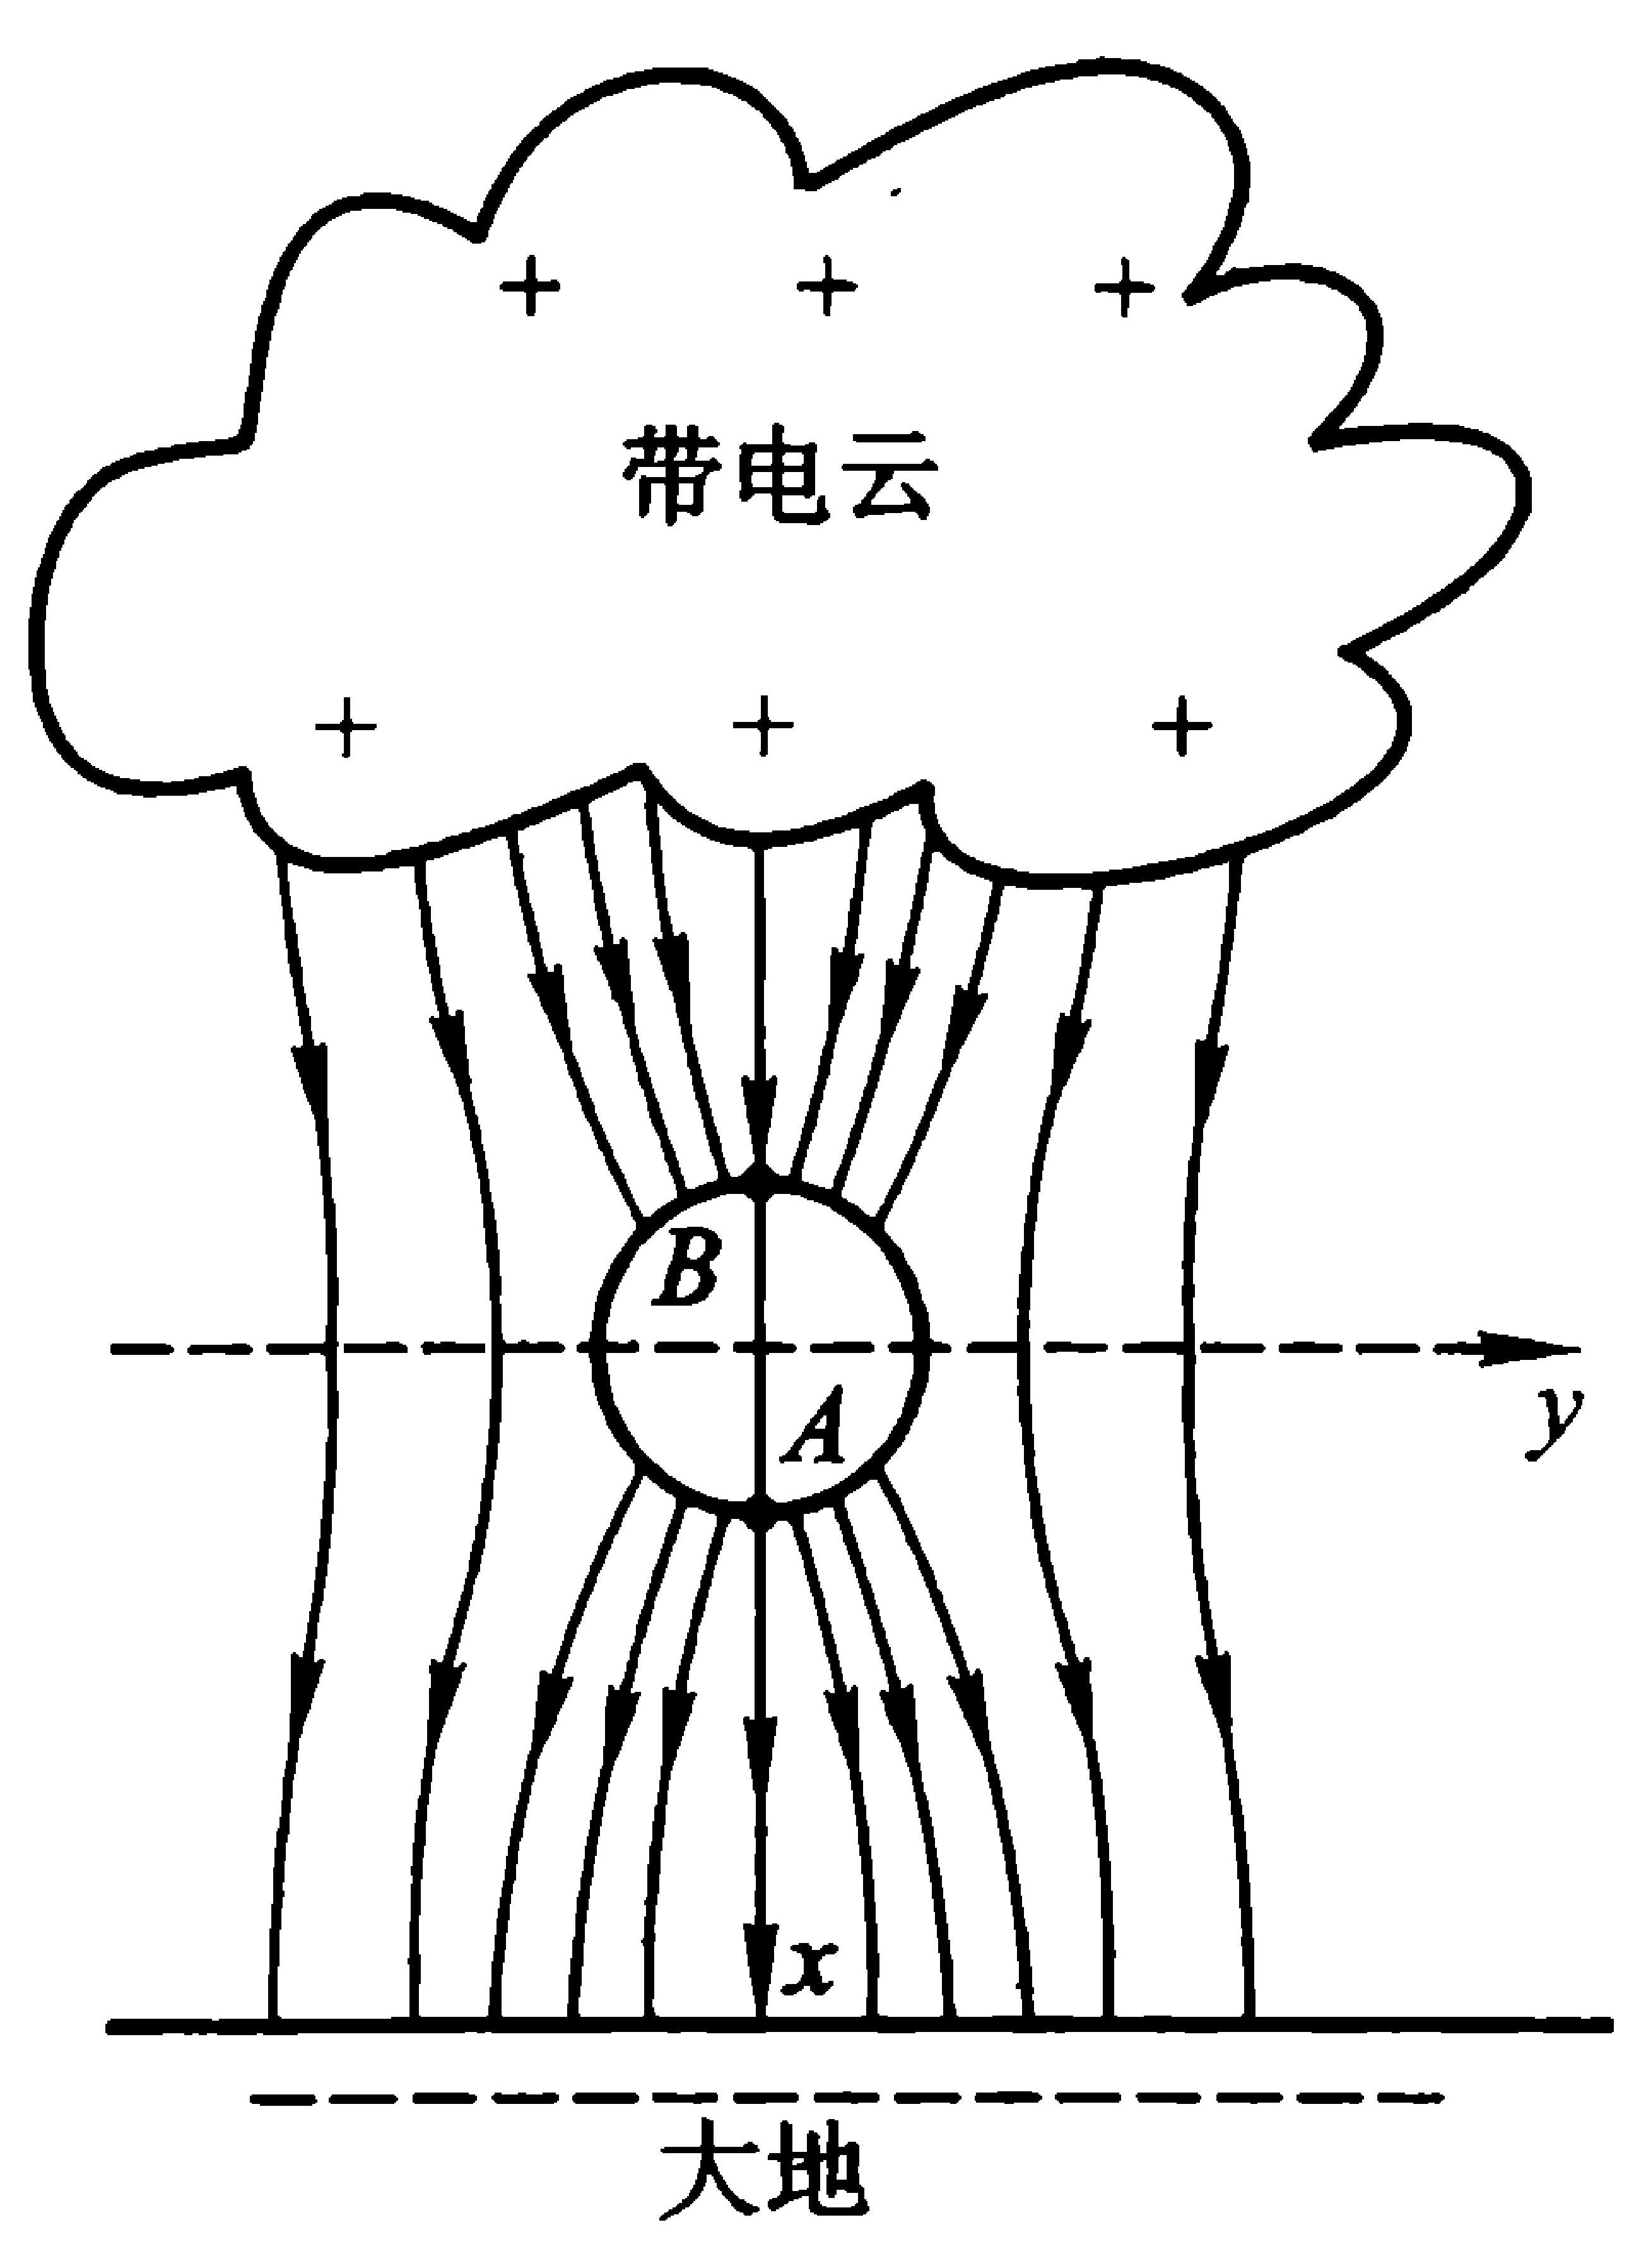
\includegraphics[width=0.3\textwidth]{wire.jpg}
    \end{center}
    \vspace{-20pt}
    \caption{输电线示意图.}
    \vspace{-10pt}
    \label{fig:wire}
  \end{wrapfigure}
首先需要把这个物理问题表为定解问题. 取圆柱的轴为 $z$ 轴. 
如果圆柱 “无限长”, 那么, 这个静电场的电场强度、电势显然跟 $z$ 无关, 我们只需在 $x y$ 平面上加以研究就够了.
图\ref{fig:wire}画的正是 $xy$ 平面上的静电场, 圆柱面在
$xy$ 平面的剖口是圆 $x^{2}+y^{2}=a^{2}$, 其中 $a$ 是圆柱的半径.

柱外的空间中没有电荷, 所以电势 $u$ 满足二维的拉普拉斯方程

$$
u_{x x}+u_{y y}=0 \quad \text { (柱外). }
$$

导体中的电荷既然不再移动, 这说明导体中各处电势相同. 又因为电势只具有相对的意义, 不妨把电势的零点取在导体上, 从而写出边界条件

$$
\left.u\right|_{x^{2}+y^{2}=a^{2}}=0 .
$$

按照分离变数法, 以 $u(x, y)=X(x) Y(y)$ 代入拉普拉斯方程固然不难把它分解为两个常微分方程,但代入上述边界条件却只能得到

$$
X(x) Y\left(\sqrt{a^{2}-x^{2}}\right)=0
$$
不能分解为 $X(x)$ 或 $Y(y)$ 的边界条件. 事实上, 既然边界是圆, 直角坐标系显然是不适当的, 必须采用平面极坐标系.

“柱外空间中的电势 $u$ 满足拉普拉斯方程” 就表为
\begin{equation}
    \frac{\partial^{2} u}{\partial \rho^{2}}+\frac{1}{\rho} \frac{\partial u}{\partial \rho}+
    \frac{1}{\rho^{2}} \frac{\partial^{2} u}{\partial \varphi^{2}}=0 \quad(\rho>a)
    \label{eq:laplace_2d}
\end{equation}
式中 $\rho$ 是极径, $\varphi$ 是极角. “导体电势为零” 就表为齐次的边界条件
\begin{equation}
    \left.u\right|_{\rho=a}=0 .
    \label{eq:laplace_2d_bc}
\end{equation}


在 “无限远” 处的静电场仍然保持为匀强的 $\bE_{0}$. 由于选取了 $x$ 轴平行于 
$\bE_{0}$, 所以在无限远处, $E_{y}=0, E_{x}=E_{0}$, 即 $-\partial u / \partial x=E_{0}$, 
亦即 $u=-E_{0} x=$ $-E_{0} \rho \cos \varphi$. 另外, 导体圆柱还可能带电, 
若单位长度导体带的电量为 $q_{0}$, 它在圆柱外产生的电势为 $\left(q_{0} / 2 \pi \varepsilon_{0}\right) \ln (1 / \rho)$, 
因而还有一个非齐次的边界条件

\begin{equation}
    \left.u\right|_{\rho \rightarrow \infty} \sim u_{0}+
    \frac{q_{0}}{2 \pi \varepsilon_{0}} \ln \frac{1}{\rho}-E_{0} \rho \cos \varphi
    \label{eq:u_rho_infty}
\end{equation}
其中 $u_{0}$ 为常数, 其数值跟电势的零点选取有关. 这里要求其满足在圆柱导体侧面上电势为零. 
问题归结为求解平面极坐标系定解问题 \eqref{eq:laplace_2d}, \eqref{eq:laplace_2d_bc}.

按照前面的步骤, 以分离变数形式的试探解
$$
u(\rho, \varphi)=R(\rho) \Phi\left(\varphi\right)
$$
代入拉普拉斯方程\eqref{eq:laplace_2d}, 得
$$
\frac{\rho}{R} \cdot \frac{d}{d \rho}\left(\rho \frac{d R}{d \rho}\right)=-\frac{\Phi^{\prime \prime}}{\Phi}
$$

上式左边是 $\rho$ 的函数,与 $\varphi$ 无关; 右边是 $\varphi$ 的函数,与 $\rho$ 无关.
 两边不可能相等, 除非两边实际上是同一个常数. 把这常数记作 $\lambda$,

$$
-\frac{\Phi^{\prime \prime}}{\Phi}=\lambda=\frac{\rho}{R} \cdot \frac{d}{d \rho}\left(\rho \frac{d R}{d \rho}\right)
$$

这就分解为两个常微分方程

\begin{eqnarray}
        \Phi^{\prime \prime}+\lambda \Phi &=& 0, \\
        \label{eq:Phi}
        \rho^{2} R^{\prime \prime}+\rho R^{'}-\lambda R  &=& 0.
        \label{eq:R}
\end{eqnarray}
常微分方程\eqref{eq:Phi}隐含着一个附加条件. 
事实上, 一个确定地点的极角可以加减 $2 \pi$ 的整倍数, 而电势 $u$ 在确定的地点应具确定数值, 
所以 $u(\rho, \varphi$ $+2 \pi)=u(\rho, \varphi)$ , 
即 $R(\rho) \Phi(\varphi+2 \pi)=R(\rho) \Phi(\varphi)$ ,亦即
\begin{equation}
    \Phi(\varphi+2 \pi)=\Phi(\varphi)
    \label{eq:Phi_bc}
\end{equation}
这叫做自然的周期条件. 常微分方程\eqref{eq:Phi} 与条件\eqref{eq:Phi_bc} 构成本征值问题. 
同样取 $\lambda$ 为实数, 不难求得方程的解为
\begin{equation}
\Phi(\varphi)= 
    \begin{cases}
        A \cos \sqrt{\lambda} \varphi+B \sin \sqrt{\lambda} \varphi & (\lambda>0), 
        \\ 
        A+B \varphi & (\lambda=0), 
        \\ 
        A e^{\sqrt{-\lambda \varphi}}+B e^{-\sqrt{-\lambda \varphi}} & (\lambda<0) .
    \end{cases}
\end{equation}

从而, 求得本征值
\begin{equation}
    \lambda =m^{2} \quad(m=0,1,2, \cdots) ; \\
    \label{eq:Phi_ev}
\end{equation}
和本征函数
\begin{equation}
\Phi(\varphi) = \begin{cases}A \cos m \varphi+B \sin m \varphi & (m \neq 0), \\
A & (m=0)\end{cases}
\label{eq:Phi_ef}
\end{equation}
以本征值\eqref{eq:Phi_ev}代入常微分方程\eqref{eq:R},
$$
\rho^{2} \frac{d^{2} R}{d \rho^{2}}+\rho \frac{d R}{d \rho}-m^{2} R=0
$$

这是欧拉型常微分方程, 作代换 $\rho=e^{t}$, 即 $t=\ln \rho$, 方程化为
$$
\frac{d^{2} R}{d t^{2}}-m^{2} R=0
$$
其解为

$$
R(\rho)= \begin{cases}C e^{m t}+D e^{-m t}=C \rho^{m}+D \frac{1}{\rho^{m}} & (m \neq 0) \\ C+D t=C+D \ln \rho & (m=0)\end{cases}
$$

这样, 分离变数形式的本征解是

$$
\begin{gathered}
u_{0}(\rho, \varphi)=C_{0}+D_{0} \ln \rho \\
u_{m}(\rho, \varphi)=\rho^{m}\left(A_{m} \cos m \varphi+B_{m} \sin m \varphi\right)+\rho^{-m}\left(C_{m} \cos m \varphi+D_{m} \sin m \varphi\right)
\end{gathered}
$$

拉普拉斯方程是线性的, 它的一般解应是所有本征解的叠加, 即

\begin{equation}
\begin{aligned}
u(\rho, \varphi)= & C_{0}+D_{0} \ln \rho+\sum_{m=1}^{\infty} \rho^{m}\left(A_{m} \cos m \varphi+B_{m} \sin m \varphi\right) \\
& +\sum_{m=1}^{\infty} \rho^{-m}\left(C_{m} \cos m \varphi+D_{m} \sin m \varphi\right)
\end{aligned}
\label{eq:u_rho_phi_general}
\end{equation}

为确定\eqref{eq:u_rho_phi_general} 中的系数, 把它代入边界条件. 先代入齐次边界条件\eqref{eq:laplace_2d_bc},
$$
\begin{gathered}
C_{0}+D_{0} \ln a+\sum_{m=1}^{\infty} a^{m}\left(A_{m} \cos m \varphi+B_{m} \sin m \varphi\right) \\
+\sum_{m=1}^{\infty} a^{-m}\left(C_{m} \cos m \varphi+D_{m} \sin m \varphi\right)=0
\end{gathered}
$$
一个傅里叶级数等于零, 意味着所有傅里叶系数为零, 即
$$
C_{0}+D_{0} \ln a=0, \quad a^{m} A_{m}+a^{-m} C_{m}=0, \quad a^{m} B_{m}+a^{-m} D_{m}=0
$$
由此,

$$
C_{0}=-D_{0} \ln a, \quad C_{m}=-A_{m} a^{2 m}, \quad D_{m}=-B_{m} a^{2 m}
$$

以此代入\eqref{eq:u_rho_phi_general}, 得
\begin{equation}
    \begin{aligned}
        u(\rho, \varphi)= & D_{0} \ln \frac{\rho}{a}+\sum_{m=1}^{\infty} \rho^{m}\left(A_{m} \cos m \varphi+B_{m} \sin m \varphi\right) \\
        & +\sum_{m=1}^{\infty} \rho^{-m}\left(-a^{2 m} A_{m} \cos m \varphi-a^{2 m} B_{m} \sin m \varphi\right)
        \end{aligned}
        \label{eq:u_rho_phi_2}
\end{equation}


将 \eqref{eq:u_rho_phi_2} 代入非齐次的边界条件\eqref{eq:u_rho_infty}, 在 $\rho$ 很大的地方, 有
\begin{equation}
    \begin{gathered}
        D_{0} \ln \frac{\rho}{a}+\sum_{m=1}^{\infty}\left[A_{m}\left(\rho^{m}-\frac{a^{2 m}}{\rho^{m}}\right) \cos m \varphi+B_{m}\left(\rho^{m}-\frac{a^{2 m}}{\rho^{m}}\right) \sin m \varphi\right] \\
        \sim u_{0}+\frac{q_{0}}{2 \pi \varepsilon_{0}} \ln \frac{1}{\rho}-E_{0} \rho \cos \varphi
    \end{gathered}
    \label{eq:matching}
\end{equation}
既然主要部分是 $\rho^{1}$ 项, 可见上式中不应出现 $\rho^{m}(m>1)$ 的项 (否则 $\rho^{m}$ 项就成了主要部分).这是说,
$$
A_{m}=0, B_{m}=0 . \quad(m>1)
$$

从\eqref{eq:matching}比较系数, 还能知道
$$
B_{1}=0, A_{1}=-E_{0}, D_{0}=-\frac{q_{0}}{2 \pi \varepsilon_{0}}, 
u_{0}=-D_{0} \ln a=\frac{q_{0}}{2 \pi \varepsilon_{0}} \ln a
$$
最后得柱外的静电势为

$$
u(\rho, \varphi)=\frac{q_{0}}{2 \pi \varepsilon_{0}} \ln \frac{a}{\rho}-E_{0} \rho \cos \varphi+E_{0} \frac{a^{2}}{\rho} \cos \varphi
$$

简单谈谈所得解答的物理含义. 
第一项是圆柱导体原来所带电荷在导体周围产生的电势. 
由于 $\rho>a$, 就好像是位于轴线 $\rho=0$ 上的带电导线产生的电势. 
常数 $u_{0}$ 的数值保证在圆柱导体的侧面上电势为零. 中间项正是原来的匀强静电场中的电势分布. 
最后一项, 即 $E_{0}\left(a^{2} / \rho\right) \cos \varphi$ 对于大的 $\rho$ 可以忽略,
所以它代表在圆柱邻近对匀强电场的修正, 这自然是柱面在匀强电场中产生的感应电荷形成的电势. 圆柱导体外的电场线分布见图 8-3a.

设圆柱体原来并不带电, 从而 $D_{0}=0$, 这时只含两项,

$$
u(\rho, \varphi)=-E_{0} \rho \cos \varphi+E_{0} \frac{a^{2}}{\rho} \cos \varphi
$$
$A$ 点和 $B$ 点的电场强度是
$$
E=-\left.\frac{\partial u}{\partial \rho}\right|_{\substack{\rho=a \\ \varphi=0, \pi}}
=\left.\left(E_{0} \cos \varphi+E_{0} \frac{a^{2}}{\rho^{2}} \cos \varphi\right)\right|_{\substack{\rho=a \\ \varphi=0, \pi}}
= \pm 2 E_{0}
$$
是原来的匀强电场的两倍! 所以在这两处特别容易击穿. 而且不管圆柱的半径多么小, 这个结论总是对的!

在$y$ 轴上的电势是
$$
u_{\varphi= \pm \pi / 2}=\left.\left(-E_{0} \rho \cos \varphi+E_{0} \frac{a^{2}}{\rho} \cos \varphi\right)\right|_{\varphi= \pm \pi / 2}=0
$$
跟导体圆柱的电势相同. 

非齐次方程在齐次边界上的模态展开已经写在本节前面:每个模式是一个受迫振子,连续力的响应是冲量的叠加.直角坐标系里把这件事写成傅里叶级数和冲量定理的细节见后文.非齐次边界条件的处理不做要求.

\section{第三类边界条件的本征值}
\idx{第三类边界条件}{disanleibianjie}
分离变量在第一类、第二类边界下得到的是正弦或余弦,本征值是显式的.一端固定、另一端弹性支承时,边界条件是第三类,本征值改由超越方程决定.

考虑区间 $0<x<l$ 上的问题
\begin{equation}
  X''+\lambda X=0,
  \qquad
  X(0)=0,
  \qquad
  X'(l)+h X(l)=0,
\end{equation}
其中 $h>0$.$h$ 就是定解条件里弹性支承的 $\sigma$.$\lambda\leq 0$ 时只有零解:$\lambda=0$ 给出直线,$X(0)=0$ 把它定成 $X=cx$,再由右端条件得 $c(1+hl)=0$.$\lambda=-\mu^2<0$ 给出双曲函数,同样只有零解.因此 $\lambda=\mu^2>0$,
\begin{equation}
  X(x)=\sin(\mu x).
\end{equation}
右端条件变成
\begin{equation}
  \mu\cos(\mu l)+h\sin(\mu l)=0,
  \qquad
  \tan(\mu l)=-\frac{\mu}{h}.
  \label{eq:third-kind-root}
\end{equation}
把 $\tan(\mu l)$ 和直线 $-\mu/h$ 画在同一张图上.在每个区间 $\bigl((n-\half)\pi,(n\pi)\bigr)$ 里,$n=1,2,\ldots$,正切从 $-\infty$ 升到 $0$,直线是负的,所以恰好有一个根 $\mu_n$.这些根没有初等表达式,但
\begin{equation}
  \bigl(n-\half\bigr)\pi < \mu_n l < n\pi,
\end{equation}
$n$ 很大时 $\mu_n$ 靠近 $n\pi/l$ 的左边.相应的本征函数 $\sin(\mu_n x)$ 仍按 Sturm--Liouville 理论在 $[0,l]$ 上正交.初始条件的系数照旧用这个内积来定,只是 $\mu_n$ 要先从\eqref{eq:third-kind-root}解出来.

\section{其他边界下的本征值}
\idx{本征值}{benzhengzhi}
两端固定的弦给出正弦族.换边界条件,分离常数的方程不变,变的是 $X$ 在端点上的条件,谱就换一族.下面都在 $0<x<\ell$ 上讨论 $X''+\lambda X=0$.三角函数族本身的正交和完备已经在傅里叶级数一章里证过,这里只列出分离变量要用的谱.

\subsection{可以写出来的谱}
第二类条件 $X'(0)=X'(\ell)=0$ 的非零解是余弦.$\lambda<0$ 时通解是指数,两端导数为零迫使两个系数都是零.$\lambda=0$ 时 $X=A+Bx$,$X'=B=0$,常数函数留下来.$\lambda=\omega^2>0$ 时 $X=\cos(\omega x)$ 满足左端,$X'(\ell)=0$ 要求 $\sin(\omega\ell)=0$,
\begin{equation}
  \lambda_n=\Bigl(\frac{n\pi}{\ell}\Bigr)^2,
  \qquad
  X_n=\cos\Bigl(\frac{n\pi x}{\ell}\Bigr),
  \qquad n=0,1,2,\ldots.
\end{equation}
$n=0$ 是整段一起平移的模式,热方程和波动方程里它不衰减,也不振动.

一端固定、一端自由,$X(0)=X'(\ell)=0$.$\lambda\leq 0$ 没有非零解.$\lambda=\omega^2$ 时 $X=\sin(\omega x)$,右端导数 $-\omega\cos(\omega\ell)=0$,所以 $\omega\ell=(n+\half)\pi$,
\begin{equation}
  \lambda_n=\Bigl(\frac{(n+\half)\pi}{\ell}\Bigr)^2,
  \qquad
  X_n=\sin\Bigl(\frac{(n+\half)\pi x}{\ell}\Bigr),
  \qquad n=0,1,2,\ldots.
  \label{eq:half-integer}
\end{equation}
两端对调,$X'(0)=X(\ell)=0$,同一组 $\lambda_n$,本征函数改成 $\cos\bigl((n+\half)\pi x/\ell\bigr)$.这就是半整数正弦族或余弦族.在 $[0,\ell]$ 上它们的范数仍是 $\ell/2$.

周期条件 $X(0)=X(\ell)$, $X'(0)=X'(\ell)$ 描述环或晶体原胞.$\lambda=0$ 只有常数.$\lambda>0$ 时两个独立解一起留下来,本征值二重,
\begin{equation}
  \lambda_n=\Bigl(\frac{2\pi n}{\ell}\Bigr)^2,
  \qquad
  X=\cos\Bigl(\frac{2\pi n x}{\ell}\Bigr),\;
  \sin\Bigl(\frac{2\pi n x}{\ell}\Bigr),
\end{equation}
$n=1,2,\ldots$.写成复指数 $e^{2\pi\imath n x/\ell}$,$n\in\mathbb{Z}$,每个 $n\neq 0$ 的模长相同,简并还在,只是基换了.

准周期条件把 Bloch 相位写进端点.设准动量 $\kappa\in(0,2\pi/\ell)$,
\begin{equation}
  X(\ell)=e^{\imath\kappa\ell}X(0),
  \qquad
  X'(\ell)=e^{\imath\kappa\ell}X'(0).
\end{equation}
解是 $X_n=\exp\bigl(\imath(2\pi n/\ell+\kappa)x\bigr)$,本征值 $(2\pi n/\ell+\kappa)^2$,$n\in\mathbb{Z}$,一般不再简并,本征函数也不再是实的.$\kappa=0$ 回到周期条件.$\kappa=\pi/\ell$ 是反周期,$X(\ell)=-X(0)$.自由电子在周期势里的能带,就是把这里的 $X''+\lambda X=0$ 换成 $X''+(\lambda-V(x))X=0$.

\begin{example}
左端固定、右端自由的热棒,初温 $g(x)=x$.写出温度.
\end{example}
\begin{solution}
用\eqref{eq:half-integer}.$u_t=k u_{xx}$,$u(0,t)=u_x(\ell,t)=0$.
\begin{equation}
  u(x,t)=\sum_{n=0}^{\infty}A_n
  \exp\Bigl(-k\lambda_n t\Bigr)
  \sin\Bigl(\frac{(n+\half)\pi x}{\ell}\Bigr).
\end{equation}
范数是 $\ell/2$,
\begin{equation}
  A_n=\frac{2}{\ell}\int_0^{\ell}x\sin\Bigl(\frac{(n+\half)\pi x}{\ell}\Bigr)\,\mathrm{d}x
  =\frac{2\ell(-1)^n}{(n+\half)^2\pi^2}.
\end{equation}
$t\to+\infty$ 时每一项都衰减,最低模式 $n=0$ 衰减最慢,速率是 $k\pi^2/(4\ell^2)$.
\end{solution}

\subsection{两端都是第三类}
\idx{罗宾条件}{luobin}
\begin{equation}
  X'(0)=\alpha X(0),
  \qquad
  X'(\ell)=-\beta X(\ell).
\end{equation}
$\alpha,\beta$ 同号时,弹性能的符号决定谱落在哪一边.分部积分,
\begin{equation}
  \lambda\int_0^{\ell}X^2\,\mathrm{d}x
  =\int_0^{\ell}(X')^2\,\mathrm{d}x+\alpha X(0)^2+\beta X(\ell)^2.
  \label{eq:robin-energy}
\end{equation}
因此 $\alpha\geq 0$, $\beta\geq 0$ 且不同时为零时,$\lambda>0$.令 $\lambda=\omega^2$,$X=\omega\cos(\omega x)+\alpha\sin(\omega x)$ 已经满足左端.代入右端,
\begin{equation}
  \tan(\omega\ell)=\frac{(\alpha+\beta)\omega}{\omega^2-\alpha\beta},
  \qquad
  X=\omega\cos(\omega x)+\alpha\sin(\omega x).
  \label{eq:robin-both}
\end{equation}
$\alpha,\beta\to 0$ 时根靠近 $(n-1)\pi/\ell$,回到余弦族;两者都趋于 $+\infty$ 时根靠近 $n\pi/\ell$,回到正弦族.

$\alpha$ 或 $\beta$ 为负时,弹性能可以是负的,\eqref{eq:robin-energy}不再禁止 $\lambda<0$.令 $\lambda=-\gamma^2$,$\gamma>0$,
\begin{equation}
  \tanh(\gamma\ell)=-\frac{(\alpha+\beta)\gamma}{\gamma^2+\alpha\beta},
  \qquad
  X=\gamma\cosh(\gamma x)+\alpha\sinh(\gamma x).
\end{equation}
$\lambda=0$ 是否是本征值,用直线 $X=cx+d$ 代进去:非零解存在当且仅当
\begin{equation}
  \alpha+\beta+\alpha\beta\ell=0.
  \label{eq:robin-threshold}
\end{equation}
这条双曲线把 $(\alpha,\beta)$ 平面分成若干块.把 $\alpha$ 或 $\beta$ 增大,\eqref{eq:robin-energy}的二次型只增不减,本征值因此不减.特别地 $\alpha=\beta$ 时可以把区间平移到中点,本征函数分成偶函数和奇函数.偶的一支在 $\alpha<0$ 时恰有一个负本征值,奇的一支还要求 $\alpha\ell<-2$.所以
\begin{itemize}
  \item $\alpha\geq 0$:没有负本征值;
  \item $-2<\alpha\ell<0$:恰有一个,本征函数为偶;
  \item $\alpha\ell<-2$:恰有两个,一偶一奇.
\end{itemize}
$\alpha\ell=-2$ 和 $\alpha=0$ 正好落在\eqref{eq:robin-threshold}上,零本征值出现在两块区域的边界.

\subsection{梁的横振动}
细梁的小挠度满足四阶方程
\begin{equation}
  u_{tt}+K u_{xxxx}=0, \qquad K>0.
\end{equation}
分离 $u=X(x)T(t)$ 得到 $X^{(4)}=\lambda X$, $T''+K\lambda T=0$.两端夹紧是 $X=X'=0$.能量
\begin{equation}
  \int_0^{\ell}(X'')^2\,\mathrm{d}x
\end{equation}
在这个边界下为正,所以 $\lambda=k^4>0$.通解
\begin{equation}
  X=A\cosh(kx)+B\sinh(kx)+C\cos(kx)+D\sin(kx).
\end{equation}
左端夹紧给出 $C=-A$, $D=-B$,
\begin{equation}
  X=A\bigl(\cosh(kx)-\cos(kx)\bigr)+B\bigl(\sinh(kx)-\sin(kx)\bigr).
\end{equation}
右端 $X(\ell)=X'(\ell)=0$ 是关于 $A,B$ 的齐次方程组,行列式为零化成
\begin{equation}
  \cosh(k\ell)\cos(k\ell)=1.
  \label{eq:beam-clamped}
\end{equation}
左端夹紧、右端自由时,自由端是弯矩和剪力为零,$X''(\ell)=X'''(\ell)=0$,同样的消元换成
\begin{equation}
  \cosh(k\ell)\cos(k\ell)=-1.
\end{equation}
两端都自由时谱和两端夹紧相同,但本征函数改成 $\cosh+\cos$ 与 $\sinh+\sin$ 的组合,并且 $\lambda=0$ 是二重本征值,刚体模式是 $1$ 和 $x$.

\begin{example}
说明两端夹紧时\eqref{eq:beam-clamped}的根都是正的,并且 $k\ell$ 落在 $(n\pi,(n+\half)\pi)$ 附近.
\end{example}
\begin{solution}
$\cosh(k\ell)\geq 1$,所以 $\cos(k\ell)=1/\cosh(k\ell)\in(0,1]$.$k=0$ 使 $X$ 恒为零,不是本征函数.在每个 $(2m\pi,(2m+1/2)\pi)$ 里余弦从 $1$ 降到 $0$,$1/\cosh$ 从略小于 $1$ 降到更小的正数,恰有一个交点.$(2m+3/2)\pi$ 到 $(2m+2)\pi$ 里余弦从 $0$ 升到 $1$,又有一个交点.大 $k$ 时 $1/\cosh$ 几乎是零,根靠近余弦的零点,也就是半整数个 $\pi$.
\end{solution}

\section{热方程的分离变量}
\idx{热方程}{refangcheng}
$u_t=k u_{xx}$,两端为零,$u(x,0)=g(x)$.分离后 $T'=-k\lambda T$,时间因子是衰减指数,不是振动,
\begin{equation}
  u(x,t)=\sum_{n=1}^{\infty}A_n e^{-k(n\pi/\ell)^2 t}
  \sin\Bigl(\frac{n\pi x}{\ell}\Bigr),
  \qquad
  A_n=\frac{2}{\ell}\int_0^{\ell}g(x)\sin\Bigl(\frac{n\pi x}{\ell}\Bigr)\,\mathrm{d}x.
  \label{eq:heat-series}
\end{equation}
$t<0$ 时指数变成增长,高模式放得最大,初值问题向过去不适定.$t\to+\infty$ 时
\begin{equation}
  u(x,t)=A_1 e^{-k\pi^2 t/\ell^2}\sin\Bigl(\frac{\pi x}{\ell}\Bigr)
  +O\bigl(e^{-4k\pi^2 t/\ell^2}\bigr).
\end{equation}
最低模式决定长时间的形状.

若方程和边界都不随时间变化,
\begin{equation}
  u_t=k u_{xx}+f(x),
  \qquad u(0,t)=\varphi, \quad u(\ell,t)=\psi,
\end{equation}
先丢掉初值,求稳态 $v''=-f/k$, $v(0)=\varphi$, $v(\ell)=\psi$.$u-v$ 满足齐次边界,按\eqref{eq:heat-series}衰减,所以
\begin{equation}
  u(x,t)=v(x)+O\bigl(e^{-k\pi^2 t/\ell^2}\bigr).
\end{equation}
温度趋于稳态.两端若改成齐次诺伊曼或周期条件,$\lambda_1=0$,常数模式不衰减.这时稳态存在的条件是总热流为零:两端诺伊曼 $u_x(0)=\varphi$, $u_x(\ell)=\psi$ 时
\begin{equation}
  \frac{1}{k}\int_0^{\ell}f\,\mathrm{d}x-\varphi+\psi=0,
\end{equation}
周期条件时积分本身必须是零.热流不平衡时,多出来的热量均匀堆积,$u=pt+A_1+O(e^{-k\lambda_2 t})$,$p$ 是 $f$ 的平均值.

\begin{example}
$u_t=u_{xx}$, $0<x<1$, $u(0,t)=0$, $u(1,t)=1$, $u(x,0)=0$.
\end{example}
\begin{solution}
稳态是 $v=x$.令 $w=u-x$,则 $w_t=w_{xx}$, $w(0,t)=w(1,t)=0$, $w(x,0)=-x$.
\begin{equation}
  A_n=2\int_0^1(-x)\sin(n\pi x)\,\mathrm{d}x=\frac{2(-1)^n}{n\pi},
\end{equation}
\begin{equation}
  u(x,t)=x+\sum_{n=1}^{\infty}\frac{2(-1)^n}{n\pi}e^{-n^2\pi^2 t}\sin(n\pi x).
\end{equation}
$t\to+\infty$ 时级数消失,温度变成线性分布 $x$.
\end{solution}

\section{薛定谔方程与零本征值的时间因子}
有限区间上的自由薛定谔方程 $u_t=\imath k u_{xx}$,边界仍是分离变量能接受的那几类.空间本征值照旧,$T'=-\imath k\lambda T$,
\begin{equation}
  u(x,t)=\sum_n A_n e^{-\imath k\lambda_n t}X_n(x).
\end{equation}
指数的模是 $1$.向过去和向未来都适定,但没有热方程那种趋于稳态的衰减.

波动方程 $u_{tt}=c^2 u_{xx}$ 在同一组 $X_n$ 上,
\begin{equation}
  T_n(t)=
  \begin{cases}
    A_n\cos(c\sqrt{\lambda_n}\,t)+B_n\sin(c\sqrt{\lambda_n}\,t), & \lambda_n>0,\\
    A_n+B_n t, & \lambda_n=0,\\
    A_n\cosh(c\sqrt{-\lambda_n}\,t)+B_n\sinh(c\sqrt{-\lambda_n}\,t), & \lambda_n<0.
  \end{cases}
\end{equation}
$\lambda=0$ 的线性项是刚体漂移,出现在两端自由或周期条件里.$\lambda<0$ 的双曲函数随时间增长,对应弹性支承吸能、平衡不稳定.系数仍由 $u(x,0)$ 和 $u_t(x,0)$ 的展开定,$B_n$ 在三种情形下分别除以 $c\sqrt{\lambda_n}$、$1$ 和 $c\sqrt{-\lambda_n}$.

\section{半带和矩形}
\idx{半带}{bandai}
半带 $0<x<\ell$, $y>0$ 上 $\Delta u=0$,左右是齐次边界,底边 $u(x,0)=g(x)$,并且 $u$ 有界.分离后 $X$ 仍是上面的本征函数,$Y''=\lambda Y$.$\lambda_n>0$ 时 $e^{\sqrt{\lambda_n} y}$ 无界,丢掉,
\begin{equation}
  u(x,y)=\sum_n A_n e^{-\sqrt{\lambda_n}\,y}X_n(x),
\end{equation}
$A_n$ 是 $g$ 的系数.若在 $y=0$ 再指定 $u_y$,两个指数都要留下,高频模式会被放大,柯西问题不适定.$\lambda=0$ 时 $Y=A+By$,有界解只能留常数.四周都是诺伊曼条件时,解存在还要求 $\int g X_0\,\mathrm{d}x=0$.

矩形 $0<x<a$, $0<y<b$,左右齐次,上下给定 $u(x,0)=g(x)$, $u(x,b)=h(x)$.两个指数都留在有限区间里,把它们收成双曲正弦后在端点取到 $1$,
\begin{equation}
  u(x,y)=\sum_n
  \Biggl(
    g_n\frac{\sinh\bigl(\sqrt{\lambda_n}(b-y)\bigr)}{\sinh(\sqrt{\lambda_n}b)}
    +h_n\frac{\sinh(\sqrt{\lambda_n}y)}{\sinh(\sqrt{\lambda_n}b)}
  \Biggr)X_n(x).
  \label{eq:rectangle-sinh}
\end{equation}
上下也改成诺伊曼、并且 $\lambda_0=0$ 时,解存在的条件是上下边界的总通量互相抵消.四边都是诺伊曼时,存在条件是四条边上的法向导数积分和为零,也就是没有净热流.函数 $v=x^2-y^2$ 本身调和,可以用来把两条边上的相容条件和另外两条拆开,再叠加回去.

\begin{example}
$0<x<\pi$, $0<y<b$, $u(0,y)=u(\pi,y)=u(x,0)=0$, $u(x,b)=\sin x$.
\end{example}
\begin{solution}
左右为零,所以 $X_n=\sin(nx)$, $\lambda_n=n^2$.顶边只有 $n=1$.\eqref{eq:rectangle-sinh}只剩一项,
\begin{equation}
  u(x,y)=\frac{\sinh y}{\sinh b}\sin x.
\end{equation}
底边 $\sinh 0=0$,顶边比值是 $1$.直接计算 $\Delta u=0$.
\end{solution}

\section{矩形域上的乘积解}
矩形膜 $0<x<a$, $0<y<b$,四周固定,$u_{tt}=c^2\Delta u$.令 $u=X(x)Y(y)T(t)$,三个变量各自成常数,
\begin{equation}
  X''+\lambda X=0, \quad Y''+\mu Y=0, \quad T''+c^2(\lambda+\mu)T=0.
\end{equation}
四周为零给出
\begin{equation}
  \lambda_m=\Bigl(\frac{m\pi}{a}\Bigr)^2, \quad
  \mu_n=\Bigl(\frac{n\pi}{b}\Bigr)^2, \quad
  \omega_{mn}=c\pi\sqrt{\frac{m^2}{a^2}+\frac{n^2}{b^2}},
\end{equation}
$m,n\geq 1$.一般解是
\begin{equation}
  u=\sum_{m,n}\bigl(A_{mn}\cos\omega_{mn}t+B_{mn}\sin\omega_{mn}t\bigr)
  \sin\Bigl(\frac{m\pi x}{a}\Bigr)\sin\Bigl(\frac{n\pi y}{b}\Bigr).
\end{equation}
热方程把 $\cos$ 和 $\sin$ 换成 $e^{-k(\lambda_m+\mu_n)t}$.长方体是同一件事再乘一个 $z$ 方向的正弦.正方形 $a=b$ 时 $\omega_{mn}=\omega_{nm}$,不同的 $(m,n)$ 可以共用一个频率.

稳态问题 $\Delta u=0$ 不能让 $\lambda$ 和 $\mu$ 同时为正又同时满足四边为零,否则 $T$ 的角色由一个会在某个方向上指数增长的因子扮演.四边为零的调和函数只有 $u=0$.非齐次边界才用上一节的双曲正弦.

\section{不先分离变量的展开}
有的方程对 $x$ 和 $t$ 分离不开,边界却仍然挑出正弦族.这时先把未知函数按这条边界允许的基展开,系数是 $t$ 的函数.

\begin{example}
$u_{tt}-2a u_{tx}-u_{xx}=0$, $0<x<\pi$, $u(0,t)=u(\pi,t)=0$.
\end{example}
\begin{solution}
试 $u=e^{\imath k(t-ax)}\sin(nx)$.代入后 $\sin(nx)$ 的系数是 $n^2-k^2(1+a^2)$.它为零时
\begin{equation}
  k=\pm\frac{n}{\sqrt{1+a^2}}, \qquad n=1,2,\ldots.
\end{equation}
两端的正弦自动满足边界.一般解是这两支的叠加,
\begin{equation}
  u=\sum_{n=1}^{\infty}
  \Bigl(
    A_n\cos\frac{n(t-ax)}{\sqrt{1+a^2}}
    +B_n\sin\frac{n(t-ax)}{\sqrt{1+a^2}}
  \Bigr)\sin(nx).
\end{equation}
$t=0$ 时 $e^{0}=1$,$A_n,B_n$ 仍由初值的正弦系数定.相因子 $t-ax$ 是输运项 $u_{tx}$ 留下的,普通的 $X(x)T(t)$ 乘积接不住它.
\end{solution}

矩形上的双调和方程 $\Delta^2 u=0$,若 $x=0,\pi$ 上 $u=u_{xx}=0$,同样可以先写 $u=\sin(nx)Y(y)$.$Y$ 满足 $(D^2-n^2)^2 Y=0$,通解是 $(A+By)e^{ny}+(C+Dy)e^{-ny}$,再由 $y$ 方向的两个边界条件定系数.

\section{多重傅里叶级数}
每个变量各自以 $2\pi$ 为周期时,系数可以一个变量一个变量地算.二元情形
\begin{equation}
  u(x,y)=\sum_{m,n\in\mathbb{Z}}c_{mn}e^{\imath(mx+ny)},
  \qquad
  c_{mn}=\frac{1}{(2\pi)^2}\int_0^{2\pi}\int_0^{2\pi}
  u(x,y)e^{-\imath(mx+ny)}\,\mathrm{d}x\,\mathrm{d}y.
\end{equation}
帕塞瓦尔等式是 $\sum|c_{mn}|^2=(2\pi)^{-2}\iint|u|^2$.格子 $\Gamma$ 换成一般的周期格时,先把基本胞腔线性变到立方体,对偶格 $\Gamma^*$ 上的波矢代替 $(m,n)$.分离变量在矩形上得到的正弦乘积,就是这个级数在齐次边界下的特例.

\section{行波法与达朗贝尔公式}
\idx{达朗贝尔公式}{dalangbei}
有界区间上的振动用分离变量最直接.无界弦上没有边界把波数离散化,通解是沿特征线传播的两列行波,初值问题的解写成达朗贝尔公式.

\subsection{一维波动方程的通解}
齐次方程
\begin{equation}
  \frac{\partial^2 u}{\partial t^2}-a^2\frac{\partial^2 u}{\partial x^2}=0,
  \qquad -\infty<x<\infty,
\end{equation}
里的 $a>0$ 是波速.引入特征坐标
\begin{equation}
  \xi=x-at, \qquad \eta=x+at.
\end{equation}
链式法则给出
\begin{align}
  u_x &= u_\xi+u_\eta, &
  u_{xx} &= u_{\xi\xi}+2u_{\xi\eta}+u_{\eta\eta}, \\
  u_t &= -a u_\xi+a u_\eta, &
  u_{tt} &= a^2 u_{\xi\xi}-2a^2 u_{\xi\eta}+a^2 u_{\eta\eta}.
\end{align}
因此
\begin{equation}
  u_{tt}-a^2 u_{xx}=-4a^2 u_{\xi\eta}.
\end{equation}
方程等价于 $u_{\xi\eta}=0$.对 $\eta$ 积分,$u_\xi$ 只依赖于 $\xi$;再对 $\xi$ 积分,
\begin{equation}
  u(x,t)=f(x-at)+g(x+at).
  \label{eq:traveling-wave}
\end{equation}
$f(x-at)$ 是以速度 $a$ 向右传播的波形,$g(x+at)$ 向左.波形本身在传播中不变形,这是无色散一维波动方程的特点.

\subsection{达朗贝尔公式}
初值
\begin{equation}
  u(x,0)=\varphi(x), \qquad u_t(x,0)=\psi(x)
\end{equation}
定出 $f$ 和 $g$.由\eqref{eq:traveling-wave},
\begin{equation}
  f(x)+g(x)=\varphi(x),
  \qquad
  -a f'(x)+a g'(x)=\psi(x).
\end{equation}
把第二式从 $0$ 积到 $x$,
\begin{equation}
  -f(x)+g(x)=\frac{1}{a}\int_0^x\psi(s)\,\mathrm{d}s+C,
\end{equation}
常数 $C=-f(0)+g(0)$.与 $f+g=\varphi$ 联立,
\begin{align}
  f(x)&=\half\varphi(x)-\frac{1}{2a}\int_0^x\psi(s)\,\mathrm{d}s-\half C, \\
  g(x)&=\half\varphi(x)+\frac{1}{2a}\int_0^x\psi(s)\,\mathrm{d}s+\half C.
\end{align}
代回 $u=f(x-at)+g(x+at)$,常数相消,得到达朗贝尔公式
\begin{equation}
  u(x,t)
  =\frac{\varphi(x-at)+\varphi(x+at)}{2}
  +\frac{1}{2a}\int_{x-at}^{x+at}\psi(s)\,\mathrm{d}s.
  \label{eq:dalembert}
\end{equation}
$t<0$ 时公式仍然成立,积分限自动交换.

点 $(x,t)$ 的位移只依赖区间 $[x-at,x+at]$ 上的初值.扰动的传播速度不超过 $a$.过该点的两条特征线 $x\pm at=\textrm{常数}$ 在 $t=0$ 上切出的这段区间,称为这个点的依赖区间.

\begin{example}
无限长弦的初位移是 $\varphi(x)=e^{-x^2}$,初速度 $\psi=0$.
\end{example}
\begin{solution}
由\eqref{eq:dalembert},
\begin{equation}
  u(x,t)=\half\left[e^{-(x-at)^2}+e^{-(x+at)^2}\right].
\end{equation}
$t=0$ 时两包重合,高度为 $1$.之后它分成向左、向右各一个高斯包,每个包的高度是 $\half$,形状不再改变.
\end{solution}

\begin{example}
初速度仍为零,初位移是宽度为 $2b$ 的矩形:$\varphi(x)=1$（$|x|<b$）,其余为 $0$.
\end{example}
\begin{solution}
$u(x,t)$ 等于 $\half$,如果 $x-at$ 和 $x+at$ 里恰有一个落在 $(-b,b)$ 内;等于 $1$,如果两个都落在里面;否则为 $0$.间断点沿着 $x=\pm b\pm at$ 四条特征线传播.某个固定的 $x$,在右行间断和左行间断先后经过之后,位移回到 $0$.一维波动方程没有尾巴:波阵面过去以后,该点可以恢复静止.
\end{solution}

\subsection{半无限弦}
弦占据 $x\geq 0$,固定端 $u(0,t)=0$.把初值奇延拓到整个直线,
\begin{equation}
  \Phi(-x)=-\Phi(x), \qquad \Psi(-x)=-\Psi(x),
\end{equation}
再套\eqref{eq:dalembert}.奇函数的组合在 $x=0$ 上自动为零.当 $x\geq at\geq 0$ 时,积分限都在正半轴,公式和无限弦相同,左行波还没有碰到端点.当 $0\leq x<at$ 时,$x-at<0$,奇延拓把它换成反射波,
\begin{equation}
  u(x,t)
  =\frac{-\varphi(at-x)+\varphi(x+at)}{2}
  +\frac{1}{2a}\int_{at-x}^{x+at}\psi(s)\,\mathrm{d}s.
\end{equation}
固定端把入射波变成反相的反射波.

\subsection{非齐次方程}
外力 $f(x,t)$ 放在右边,
\begin{equation}
  u_{tt}-a^2 u_{xx}=f(x,t).
\end{equation}
先看零初值.固定 $\tau$,令 $v(x,t;\tau)$ 满足齐次波动方程,并且
\begin{equation}
  v(x,\tau;\tau)=0, \qquad v_t(x,\tau;\tau)=f(x,\tau).
\end{equation}
这是从时刻 $\tau$ 开始的达朗贝尔问题,时间间隔是 $t-\tau$,
\begin{equation}
  v(x,t;\tau)
  =\frac{1}{2a}\int_{x-a(t-\tau)}^{x+a(t-\tau)} f(s,\tau)\,\mathrm{d}s,
  \qquad t\geq\tau.
\end{equation}
把各时刻的冲量叠加,
\begin{equation}
  u(x,t)=\int_0^t v(x,t;\tau)\,\mathrm{d}\tau
  =\frac{1}{2a}\int_0^t\mathrm{d}\tau
    \int_{x-a(t-\tau)}^{x+a(t-\tau)} f(s,\tau)\,\mathrm{d}s.
  \label{eq:duhamel-wave}
\end{equation}
$t=0$ 时积分为零,所以 $u(x,0)=0$.对上限和被积函数用莱布尼茨法则,$u_t(x,0)=0$,并且 $u_{tt}-a^2 u_{xx}=f$.一般初值只要把\eqref{eq:dalembert}和\eqref{eq:duhamel-wave}相加.这个叠加称为齐次化原理,也就是波动方程的 Duhamel 原理.

\subsection{三维波动方程}
三维齐次方程 $u_{tt}=a^2\Delta u$ 的初值解由球面上的平均给出.记
\begin{equation}
  M_R[\varphi](\br)
  =\frac{1}{4\pi R^2}\int_{|\brp-\br|=R}\varphi(\brp)\,\mathrm{d}S'.
\end{equation}
泊松公式是
\begin{equation}
  u(\br,t)
  =\funcpd{}{t}\bigl(t\, M_{at}[\varphi]\bigr)
  +t\, M_{at}[\psi].
  \label{eq:poisson-wave}
\end{equation}
右端只取半径正好等于 $at$ 的球面.三维空间里,波阵面经过之后该点立刻恢复到波前的状态,这是惠更斯原理.二维波动方程的依赖区域是整个圆盘而不只是圆周,波阵面过去以后还有余振.一维公式\eqref{eq:dalembert}里的积分填满整段区间,也有这种尾巴;矩形初位移那个例子里尾巴刚好是零,是因为 $\varphi$ 在波阵面之间取常值.

\section{积分变换法}
无界或半无界区域上,边界不把谱离散成级数.对那个无限延伸的变量作积分变换,可以把偏微分方程降成常微分方程.这里的傅里叶变换采用性质一节里的对称约定
\begin{equation}
  F(\omega)=\frac{1}{\sqrt{2\pi}}\int_{-\infty}^{\infty} f(x)\,e^{-\imath\omega x}\,\mathrm{d}x,
  \qquad
  f(x)=\frac{1}{\sqrt{2\pi}}\int_{-\infty}^{\infty} F(\omega)\,e^{\imath\omega x}\,\mathrm{d}\omega.
\end{equation}
导数定理是 $\mathcal{F}[f']=\imath\omega F$,卷积定理是 $\mathcal{F}[f_1*f_2]=\sqrt{2\pi}\,F_1 F_2$.

\subsection{热传导与高斯核}
无限长细杆
\begin{equation}
  \frac{\partial u}{\partial t}=a^2\frac{\partial^2 u}{\partial x^2},
  \qquad
  u(x,0)=\varphi(x),
\end{equation}
$a^2$ 是扩散系数.对 $x$ 作傅里叶变换,$\mathcal{F}[u_{xx}]=(\imath\omega)^2 U=-\omega^2 U$,于是
\begin{equation}
  \frac{\partial U}{\partial t}=-a^2\omega^2 U,
  \qquad
  U(\omega,t)=\Phi(\omega)\,e^{-a^2\omega^2 t}.
\end{equation}
设核 $K$ 的像函数满足 $\sqrt{2\pi}\,\widehat K=e^{-a^2\omega^2 t}$,则 $U=\sqrt{2\pi}\,\widehat K\,\Phi$ 正好是卷积定理的右边,$u=K*\varphi$.令 $\beta=a^2 t$,
\begin{equation}
  \widehat K(\omega)=\frac{1}{\sqrt{2\pi}}e^{-\beta\omega^2}.
\end{equation}
逆变换是高斯积分,
\begin{equation}
  K(x,t)
  =\frac{1}{2\pi}\int_{-\infty}^{\infty} e^{-\beta\omega^2+\imath\omega x}\,\mathrm{d}\omega
  =\frac{1}{\sqrt{4\pi a^2 t}}
    \exp\Bigl(-\frac{x^2}{4a^2 t}\Bigr),
  \qquad t>0.
  \label{eq:heat-kernel}
\end{equation}
因此
\begin{equation}
  u(x,t)
  =\int_{-\infty}^{\infty} K(x-y,t)\,\varphi(y)\,\mathrm{d}y.
  \label{eq:heat-convolution}
\end{equation}
$K$ 对 $x$ 的积分是 $1$,总热量守恒.$t\to 0^+$ 时 $K$ 趋于 $\delta(x)$,回到初值.时间越长,高斯越矮、越宽.

\begin{example}
初温 $\varphi(x)=e^{-x^2}$.
\end{example}
\begin{solution}
两个高斯的卷积仍是高斯.直接用像函数更快.$\varphi$ 对应上面傅里叶变换例子里的 $\alpha=1$,
\begin{equation}
  \Phi(\omega)=\frac{1}{\sqrt{2}}e^{-\omega^2/4},
\end{equation}
\begin{equation}
  U(\omega,t)=\frac{1}{\sqrt{2}}
  \exp\Bigl(-\frac{\omega^2}{4}(1+4a^2 t)\Bigr).
\end{equation}
对照 $e^{-\alpha x^2}$ 的像函数 $e^{-\omega^2/(4\alpha)}/\sqrt{2\alpha}$,这里 $1/(4\alpha)=(1+4a^2 t)/4$,即 $\alpha=1/(1+4a^2 t)$,并且系数 $1/\sqrt{2}$ 比 $1/\sqrt{2\alpha}$ 少一个因子 $\sqrt{\alpha}$.所以
\begin{equation}
  u(x,t)=\frac{1}{\sqrt{1+4a^2 t}}
  \exp\Bigl(-\frac{x^2}{1+4a^2 t}\Bigr).
\end{equation}
\end{solution}

\subsection{拉普拉斯变换}
半无限杆 $x>0$ 的一端温度给定、初温为零时,对时间作拉普拉斯变换更合适.设
\begin{equation}
  u_t=a^2 u_{xx},
  \qquad
  u(x,0)=0,
  \qquad
  u(0,t)=T_0,
  \qquad
  u(\infty,t)\ \textrm{有界}.
\end{equation}
记 $\bar u(x,p)=\int_0^{\infty} e^{-pt}u(x,t)\,\mathrm{d}t$.零初值使 $u_t$ 的像是 $p\bar u$,
\begin{equation}
  a^2\frac{\mathrm{d}^2\bar u}{\mathrm{d}x^2}-p\bar u=0,
  \qquad
  \bar u(0,p)=\frac{T_0}{p}.
\end{equation}
有界解是
\begin{equation}
  \bar u(x,p)=\frac{T_0}{p}\exp\Bigl(-\frac{x}{a}\sqrt{p}\Bigr).
\end{equation}
$\mathcal{L}\{\operatorname{erfc}(k/(2\sqrt{t}))\}=e^{-k\sqrt{p}}/p$,因此
\begin{equation}
  u(x,t)=T_0\operatorname{erfc}\Bigl(\frac{x}{2a\sqrt{t}}\Bigr).
\end{equation}
$t\to 0^+$ 时,只要 $x>0$,自变量趋于无穷,$\operatorname{erfc}$ 趋于 $0$,与零初温一致.$x=0$ 处 $\operatorname{erfc}(0)=1$,端点保持 $T_0$.热量从端面逐渐渗进杆内.

若把条件改成 $u(x,0)=T_0$、$u(0,t)=0$,解是 $T_0\operatorname{erf}\bigl(x/(2a\sqrt{t})\bigr)$.它和上一个解相加等于 $T_0$,因为常值函数是热方程的解,而 $\operatorname{erf}+\operatorname{erfc}=1$.

\subsection{同时变换两个变量}
对流热传导
\begin{equation}
  u_t+b u_x=a^2 u_{xx},
  \qquad
  u(x,0)=\varphi(x),
\end{equation}
先对 $x$ 作傅里叶变换.$\mathcal{F}[u_x]=\imath\omega U$,
\begin{equation}
  U_t+(\imath b\omega+a^2\omega^2)U=0,
\end{equation}
\begin{equation}
  U(\omega,t)=\Phi(\omega)\,e^{-a^2\omega^2 t}\,e^{-\imath b\omega t}.
\end{equation}
后一个因子是延迟定理:它把热核的中心从 $x$ 挪到 $x-bt$.解是
\begin{equation}
  u(x,t)=\int_{-\infty}^{\infty} K(x-bt-y,t)\,\varphi(y)\,\mathrm{d}y,
\end{equation}
$K$ 仍是\eqref{eq:heat-kernel}.扩散在以速度 $b$ 移动的坐标系里进行.

若方程再加一个线性衰减 $-cu$,像函数多一个因子 $e^{-ct}$,温度整体按 $e^{-ct}$ 衰减,空间形状不变.有源项 $f(x,t)$ 则在像函数上变成非齐次一阶方程,解出来是热核关于时间的 Duhamel 积分
\begin{equation}
  u(x,t)=\int_0^t\mathrm{d}\tau\int_{-\infty}^{\infty}
  K(x-y,t-\tau)\,f(y,\tau)\,\mathrm{d}y,
\end{equation}
这里写的是 $b=c=0$、零初温的情形.

方程要连同定解条件一起写.分离变量的系数不算完,就不能算这道题做完.

\begin{problemset}
\renewcommand{\theenumi}{\thechapter.\arabic{enumi}}
\renewcommand{\labelenumi}{\theenumi.}
\item 由牛顿定律写出两端张力为 $T$、线密度为 $\rho$ 的横振动方程,并指出波速 $a$ 与 $T,\rho$ 的关系.说明固定端和自由端分别对应哪一类边界条件.

\item 判断下列方程的类型,并说明哪一类数据是适当的: $u_{tt}-a^2 u_{xx}=0$, $u_t-a^2 u_{xx}=0$, $u_{xx}+u_{yy}=0$.

\item 无界弦 $u_{tt}-a^2 u_{xx}=0$, $u(x,0)=\sin(kx)$, $u_t(x,0)=0$.用达朗贝尔公式写出 $u(x,t)$,并验证它满足方程和初值.

\item 两端固定的弦, $u(0,t)=u(\ell,t)=0$, $u(x,0)=\varphi(x)$, $u_t(x,0)=0$.分离变量,写出本征值和级数解.取 $\varphi(x)=x(\ell-x)$,把系数积分出来.

\item 第三类边界 $X(0)=0$, $X'(l)+hX(l)=0$, $h>0$.证明本征值由 $\tan(\mu l)=-\mu/h$ 决定,并且每个区间 $((n-1/2)\pi,n\pi)$ 里恰有一根.

\item 无限长杆 $u_t=a^2 u_{xx}$, $u(x,0)=\varphi(x)$.写出热核卷积.若 $\varphi$ 是常数 $T_0$,说明 $u$ 为什么保持为 $T_0$.

\item 在 $0<x<\ell$ 上求 $X''+\lambda X=0$ 的本征值和本征函数:两端自由;左端固定、右端自由.说明第二种情形为什么没有 $\lambda=0$.

\item 两端第三类条件 $X'(0)=\alpha X(0)$, $X'(\ell)=-\beta X(\ell)$, $\alpha,\beta\geq 0$ 且不同时为零.由能量恒等式说明 $\lambda>0$,并推出 $\tan(\omega\ell)=(\alpha+\beta)\omega/(\omega^2-\alpha\beta)$.再说明 $\alpha=\beta$ 且 $\alpha\ell<-2$ 时为什么有两个负本征值.

\item 两端夹紧的梁,$X(0)=X'(0)=X(\ell)=X'(\ell)=0$.把通解里的两个系数用左端条件消去,证明频率满足 $\cosh(k\ell)\cos(k\ell)=1$.

\item $u_t=u_{xx}$, $0<x<1$, $u(0,t)=0$, $u(1,t)=1$, $u(x,0)=0$.先求稳态,再把差按正弦级数展开.

\item 矩形 $0<x<a$, $0<y<b$ 上 $\Delta u=0$,左右和下边为零,上边是 $\sin(\pi x/a)$.写出解,并在四条边上核对.

\item 矩形膜 $0<x<a$, $0<y<b$,四周固定.写出 $u_{tt}=c^2\Delta u$ 的频率 $\omega_{mn}$.说明 $a=b$ 时哪些模式简并.

\item $u_{tt}-2a u_{tx}-u_{xx}=0$, $0<x<\pi$, $u(0,t)=u(\pi,t)=0$.用 $e^{\imath k(t-ax)}\sin(nx)$ 定出 $k$,并说明为什么普通的 $X(x)T(t)$ 乘积解不出这个方程.
\end{problemset}

% \section{定解问题}